\documentclass[prl,twocolumn,amsmath]{revtex4}

\usepackage{blindtext}

\providecommand{\point}{10000}
% htr to eV
\providecommand{\htrToEV}{27.211399}
% htr to meV
\providecommand{\htrToMeV}{27211.399}
% htr to fs
\providecommand{\htrToThz}{2.418884326505e-5}
% meV to Thz
\providecommand{\meVToTHz}{1.5192667358470382}
% G_omega from atomic units to meV / A^2 
\providecommand{\GFreq}{97172.3224386509}
% G_nu from atomic units to (meV / A)^2 
\providecommand{\GnuConv}{2644231504.6}

% shifts to align valence and conduction band relative to the Fermi energy
\providecommand{\gwFermi}{0.0167748486581}
\providecommand{\gwReVBa}{0.00093344658669}
\providecommand{\gwReCBa}{-0.000906682891342}
\providecommand{\gap}{0.23479245}
\providecommand{\gapCorr}{0.0202663100855}
\providecommand{\vbMax}{-8.75333295715961e-03}
\providecommand{\cbMin}{8.53193322468371e-03}
% shifts a = 1K, b = 50K, d = 150K
\providecommand{\modelFermi}{0.1171148183155}
\providecommand{\modelReVBa}{0.000752644202393}
\providecommand{\modelReVBb}{0.000796065134215}
\providecommand{\modelReVBc}{0.000987119897961}
\providecommand{\modelReVBd}{0.00123090789335}
\providecommand{\modelReCBa}{-0.000718208143841}
\providecommand{\modelReCBb}{-0.000759642418825}
\providecommand{\modelReCBc}{-0.000941955770614}
\providecommand{\modelReCBd}{-0.00117458962749}
% shifts a = 1K, b = 50K, d = 150K
\providecommand{\epwFermi}{-0.00011069986623795}
\providecommand{\epwReVBa}{8.30972733014433e-04}
\providecommand{\epwReVBb}{7.45813259564113e-04}
\providecommand{\epwReVBd}{7.59440107944252e-04}
\providecommand{\epwReCBa}{-3.26883292067430e-04}
\providecommand{\epwReCBb}{-7.95622173755268e-05}
\providecommand{\epwReCBd}{6.89800641335590e-04}

% access to real part
\providecommand{\rePart}{\thisrowno{3}}
\providecommand{\imPart}{\thisrowno{2}}
    
% length of b over a axis
\providecommand{\bOverA}{1.42373777302672602413}

\usepackage{pgfplots}
\usetikzlibrary{calc,3d}
\usepgfplotslibrary{groupplots}
\usepgfplotslibrary{fillbetween}
\pgfplotsset{compat=1.13}

\pgfplotsset{
%  every tick/.append style={darkgray},
  every tick label/.append style={font=\footnotesize},
  every axis legend/.append style={font=\scriptsize},
  every axis label/.append style={font=\footnotesize},
%  every major grid/.append style={color=black},
}

\pgfrealjobname{makepic}

\definecolor{altblue}{HTML}{054A6B}
\definecolor{altyellow}{HTML}{F4C61F}
\definecolor{altred}{HTML}{FF3523}
\definecolor{altgreen}{HTML}{08A045}
\definecolor{altpurple}{HTML}{4C212A}
\definecolor{altblack}{HTML}{0A0908}
\definecolor{altwhite}{HTML}{F5F6F8}

\providecommand{\vect}[1]{\ensuremath{\boldsymbol{#1}}}
\providecommand{\apex}[1]{\ensuremath{^\text{#1}}}
\providecommand{\pedex}[1]{\ensuremath{_\text{#1}}}
\providecommand{\diff}[2][]{\ensuremath{\mathop{\text{d}^{#1}{#2}}}}
\providecommand{\abs}[1]{\ensuremath\lvert#1\rvert}

\begin{document}

\begin{figure}
\beginpgfgraphicnamed{coupling}%
\begin{tikzpicture}
  \begin{groupplot}[
    group style = {
      group size = 3 by 1,
      horizontal sep = 2pt,
      y descriptions at=edge left,
    },
    ybar stacked,
    %xlabel = {$\omega_\nu\thinspace(meV)$},
    %bar width=1.2pt,
    ymin = 0, ymax = 45,
    ylabel = $G_\nu\thinspace(\text{meV}^2 / \text{\AA}^2)$,
    ylabel near ticks,
    height = 0.6\columnwidth,
    scale only axis,
    legend style = {
      draw = none,
      legend cell align = left,
    },
  ]
  \nextgroupplot[
    xmin = 9, xmax = 22,
    xtick = {10, 15, 20},
    axis y line* = left,
    bar width = 2pt,
    width = 0.381\columnwidth,
  ]
    \addplot[fill,altblue!80!white] table[x expr = {\thisrowno{17} * \htrToMeV}, y expr = {(\thisrowno{7}) / (\thisrowno{2} + \thisrowno{11}) * \thisrowno{18} * \GnuConv}] {data/coupling.dat};
    \addplot[fill,altblack] table[x expr = {\thisrowno{17} * \htrToMeV}, y expr = {(\thisrowno{12}) / (\thisrowno{2} + \thisrowno{11}) * \thisrowno{18} * \GnuConv}] {data/coupling.dat};
    \addplot[fill,altred] table[x expr = {\thisrowno{17} * \htrToMeV}, y expr = {(\thisrowno{14} + \thisrowno{15}) / (\thisrowno{2} + \thisrowno{11}) * \thisrowno{18} * \GnuConv}] {data/coupling.dat};
    \addplot[fill,altgreen] table[x expr = {\thisrowno{17} * \htrToMeV}, y expr = {(\thisrowno{16}) / (\thisrowno{2} + \thisrowno{11}) * \thisrowno{18} * \GnuConv}] {data/coupling.dat};
    \addplot[fill,gray] table[x expr = {\thisrowno{17} * \htrToMeV}, y expr = {(\thisrowno{2} - \thisrowno{7} + \thisrowno{17}) / (\thisrowno{2} + \thisrowno{11}) * \thisrowno{18} * \GnuConv}] {data/coupling.dat};
    \draw[thick] (rel axis cs:0.995,0) -- (rel axis cs:0.995,0.02);
    \draw[thick] (rel axis cs:0.995,1) -- (rel axis cs:0.995,0.98);
    \coordinate (bl) at (rel axis cs:0,0);
    
  \nextgroupplot[
    xmin = 109, xmax = 116,
    xtick = {110, 115},
    hide y axis = true,
    bar width = 2pt,
    width = 0.205\columnwidth,
  ]
    \addplot[fill,altblue!80!white] table[x expr = {\thisrowno{17} * \htrToMeV}, y expr = {(\thisrowno{7}) / (\thisrowno{2} + \thisrowno{11}) * \thisrowno{18} * \GnuConv}] {data/coupling.dat};
    \addplot[fill,altblack] table[x expr = {\thisrowno{17} * \htrToMeV}, y expr = {(\thisrowno{12}) / (\thisrowno{2} + \thisrowno{11}) * \thisrowno{18} * \GnuConv}] {data/coupling.dat};
    \addplot[fill,altred] table[x expr = {\thisrowno{17} * \htrToMeV}, y expr = {(\thisrowno{14} + \thisrowno{15}) / (\thisrowno{2} + \thisrowno{11}) * \thisrowno{18} * \GnuConv}] {data/coupling.dat};
    \addplot[fill,altgreen] table[x expr = {\thisrowno{17} * \htrToMeV}, y expr = {(\thisrowno{16}) / (\thisrowno{2} + \thisrowno{11}) * \thisrowno{18} * \GnuConv}] {data/coupling.dat};
    \addplot[fill,gray] table[x expr = {\thisrowno{17} * \htrToMeV}, y expr = {(\thisrowno{2} - \thisrowno{7} + \thisrowno{17}) / (\thisrowno{2} + \thisrowno{11}) * \thisrowno{18} * \GnuConv}] {data/coupling.dat};
    \draw[thick] (rel axis cs:0.005,0) -- (rel axis cs:0.005,0.02);
    \draw[thick] (rel axis cs:0.005,1) -- (rel axis cs:0.005,0.98);
    \draw[thick] (rel axis cs:0.995,0) -- (rel axis cs:0.995,0.02);
    \draw[thick] (rel axis cs:0.995,1) -- (rel axis cs:0.995,0.98);
    
  \nextgroupplot[
    xmin = 374, xmax = 383,
    xtick = {375, 380},
    axis y line* = right,
    bar width = 2pt,
    width = 0.264\columnwidth,
  ]
    \addplot[fill,altblue!80!white] table[x expr = {\thisrowno{17} * \htrToMeV}, y expr = {(\thisrowno{7}) / (\thisrowno{2} + \thisrowno{11}) * \thisrowno{18} * \GnuConv}] {data/coupling.dat};
    \addplot[fill,altblack] table[x expr = {\thisrowno{17} * \htrToMeV}, y expr = {(\thisrowno{12}) / (\thisrowno{2} + \thisrowno{11}) * \thisrowno{18} * \GnuConv}] {data/coupling.dat};
    \addplot[fill,altred] table[x expr = {\thisrowno{17} * \htrToMeV}, y expr = {(\thisrowno{14} + \thisrowno{15}) / (\thisrowno{2} + \thisrowno{11}) * \thisrowno{18} * \GnuConv}] {data/coupling.dat};
    \addplot[fill,altgreen] table[x expr = {\thisrowno{17} * \htrToMeV}, y expr = {(\thisrowno{16}) / (\thisrowno{2} + \thisrowno{11}) * \thisrowno{18} * \GnuConv}] {data/coupling.dat};
    \addplot[fill,gray] table[x expr = {\thisrowno{17} * \htrToMeV}, y expr = {(\thisrowno{2} - \thisrowno{7} + \thisrowno{17}) / (\thisrowno{2} + \thisrowno{11}) * \thisrowno{18} * \GnuConv}] {data/coupling.dat};
    \draw[thick] (rel axis cs:0.005,0) -- (rel axis cs:0.005,0.02);
    \draw[thick] (rel axis cs:0.005,1) -- (rel axis cs:0.005,0.98);
    \coordinate (br) at (rel axis cs:1,0);
    \legend{PbI$_3$ internal, MA translation, MA libration, MA internal, other,}
  \end{groupplot}
  \node[below=4mm] at ($0.5*(bl) + 0.5*(br)$) {\footnotesize $\omega_\nu\thinspace(\text{meV})$};
\end{tikzpicture}%
\endpgfgraphicnamed
\caption{\blindtext}
\end{figure}

%\begin{figure}
%\beginpgfgraphicnamed{coupl-freq}%
%\begin{tikzpicture}[>=stealth]
%  \tikzstyle{model}=[densely dashed,thick,->]
%%  \tikzstyle{plot}=[very thick,white,postaction={draw,gray,thin}]
%  \tikzset{plot/.style args={#1}{%
%    darkgray,fill=#1,fill opacity=0.5
%  }}
%  \begin{groupplot}[
%    group style = {
%      group size = 3 by 1,
%      horizontal sep = 2pt,
%      y descriptions at=edge left,
%    },
%    %ybar stacked,
%    %xlabel = {$\omega_\nu\thinspace(meV)$},
%    %bar width=1.2pt,
%    ymin = 0, ymax = 105,
%    ytick = {0, 20, 40, 60, 80, 100},
%    yticklabels = {0, 20, 40, 60, 80, \llap{1}00},
%    ylabel = $G(\omega)\thinspace(\text{meV}^2 / \text{\AA}^2)$,
%    ylabel near ticks,
%    height = 0.6\columnwidth,
%    scale only axis,
%    legend style = {
%      draw = none,
%      legend cell align = left,
%    },
%  ]
%  \nextgroupplot[
%    xmin = 9, xmax = 22.5,
%    xtick = {10, 15, 20},
%    axis y line* = left,
%    bar width = 2pt,
%    width = 0.376\columnwidth,
%  ]
%%    \fill[model] (axis cs:12.88,0) rectangle (axis cs:13.28,103.2);
%%    \fill[model] (axis cs:20.80,0) rectangle (axis cs:21.20, 67.3);
%    \draw[model,altblue] (axis cs:13.08,0) -- (axis cs:13.08,103.2);
%    \draw[model,altred] (axis cs:21.00,0) -- (axis cs:21.00, 67.3);
%    \addplot[plot=altblue] table[x expr = {\thisrowno{0} * \htrToMeV}, y expr = {\thisrowno{1} * \GFreq}] {data/coupl_freq1.dat};
%    \addplot[plot=altred] table[x expr = {\thisrowno{0} * \htrToMeV}, y expr = {\thisrowno{1} * \GFreq}] {data/coupl_freq2.dat};
%    \draw[thick] (rel axis cs:0.995,0) -- (rel axis cs:0.995,0.02);
%    \draw[thick] (rel axis cs:0.995,1) -- (rel axis cs:0.995,0.98);
%    \coordinate (bl) at (rel axis cs:0,0);
%    \coordinate (tl) at (rel axis cs:0,1);
%    
%  \nextgroupplot[
%    xmin = 109, xmax = 116,
%    xtick = {110, 115},
%    hide y axis = true,
%    bar width = 2pt,
%    width = 0.195\columnwidth,
%  ]
%    \addplot[plot=altgreen] table[x expr = {\thisrowno{0} * \htrToMeV}, y expr = {\thisrowno{1} * \GFreq}] {data/coupl_freq3.dat};
%    \draw[thick] (rel axis cs:0.005,0) -- (rel axis cs:0.005,0.02);
%    \draw[thick] (rel axis cs:0.005,1) -- (rel axis cs:0.005,0.98);
%    \draw[thick] (rel axis cs:0.995,0) -- (rel axis cs:0.995,0.02);
%    \draw[thick] (rel axis cs:0.995,1) -- (rel axis cs:0.995,0.98);
%    
%  \nextgroupplot[
%    xmin = 374, xmax = 383,
%    xtick = {375, 380},
%    axis y line* = right,
%    bar width = 2pt,
%    width = 0.251\columnwidth,
%  ]
%%    \fill[model] (axis cs:379.54,0) rectangle (axis cs:379.94,52.6);
%    \draw[model,altgreen] (axis cs:379.74,0) -- (axis cs:379.74,52.6);
%    \addplot[plot=altgreen] table[x expr = {\thisrowno{0} * \htrToMeV}, y expr = {\thisrowno{1} * \GFreq}] {data/coupl_freq3.dat};
%    \draw[thick] (rel axis cs:0.005,0) -- (rel axis cs:0.005,0.02);
%    \draw[thick] (rel axis cs:0.005,1) -- (rel axis cs:0.005,0.98);
%    \coordinate (br) at (rel axis cs:1,0);
%  \end{groupplot}
%  \node[below=4mm] at ($0.5*(bl) + 0.5*(br)$) {\footnotesize $\omega\thinspace(\text{meV})$};
%%  \begin{scope}[scale=0.6,shift={(2,-3)}]
%%    \sffamily
%%    \tikzstyle{octahedra} = [draw=altblack, fill=lightgray]
%%    \tikzset{atom/.style args={#1}{%
%%      draw,text=altwhite,circle,fill=#1,
%%    }}
%%    \providecommand{\iod}{node[atom=purple,text=altblack,circle] {\tiny I}}
%%    \path[octahedra] (-1,0) \iod -- (0,1) \iod -- (1,0) -- (0,-1) \iod -- cycle;
%%    \node[] {\tiny Pb};
%%    \begin{scope}[shift={(2,0)}]
%%      \path[octahedra] (-1,0) \iod -- (0,1) \iod -- (1,0) \iod -- (0,-1) \iod-- cycle;
%%      \node[] {\tiny Pb};
%%    \end{scope}
%%    \begin{scope}[shift={(0,-3.5)}]
%%      \path[octahedra] (-1.2,0) \iod -- (0,1.2) \iod -- (1.2,0) -- (0,-1.2) \iod -- cycle;
%%      \node[] {\tiny Pb};
%%    \end{scope}
%%    \begin{scope}[shift={(2,-3.5)}]
%%    \path[octahedra] (-0.8,0) \iod -- (0,0.8) \iod -- (0.8,0) \iod -- (0,-0.8) \iod -- cycle;
%%      \node[] {\tiny Pb};
%%    \end{scope}
%%    \begin{scope}[shift={(6,0)}]
%%      \node[atom=darkgray] (c1) at (0.0, 0.7) {\tiny C};
%%      \node[atom=altblue]  (n1) at (0.0,-0.7) {\tiny N};
%%      \node[atom=darkgray] (c2) at (2.0,-0.7) {\tiny C};
%%      \node[atom=altblue]  (n2) at (2.0, 0.7) {\tiny N};
%%      \draw[thick] (c1) -- (n1);
%%      \draw[thick] (c2) -- (n2);
%%    \end{scope}
%%    \begin{scope}[shift={(6,-3.5)}]
%%      \node[atom=darkgray] (c1) at (-0.15, 0.7) {\tiny C};
%%      \node[atom=altblue]  (n1) at ( 0.15,-0.7) {\tiny N};
%%      \node[atom=darkgray] (c2) at ( 1.85,-0.7) {\tiny C};
%%      \node[atom=altblue]  (n2) at ( 2.15, 0.7) {\tiny N};
%      \draw[thick] (c1) -- (n1);
%%      \draw[thick] (c2) -- (n2);
%%    \end{scope}
%%  \end{scope}
%  \begin{scope}[shift={(1.1,-3)}]
%    \node[] {\includegraphics[scale=0.05]{mode_one.png}};
%    \node[] at (4.2,0) {\includegraphics[scale=0.05]{mode_two.png}};
%  \end{scope}
%  \node[below right, inner sep = 0pt] at ($(tl) - (1,0)$) {a)};
%  \node[below right, inner sep = 0pt] at ($(tl) - (1,6)$) {b)};
%\end{tikzpicture}
%\endpgfgraphicnamed
%\caption{\blindtext}
%\end{figure}

\begin{figure}
\beginpgfgraphicnamed{coupl-freq}%
\begin{tikzpicture}[>=stealth]
  \tikzstyle{model}=[line width=1pt,->]
  \tikzstyle{connect}=[thick,dotted]
  \tikzset{plot/.style args={#1}{%
    darkgray,fill=#1,fill opacity=0.3
  }}
  \begin{axis}[
    width=0.72\columnwidth, height=0.33\columnwidth,
    xmin = 0, xmax = 25,
    xlabel = {$\hbar\omega\thinspace(\text{meV})$},
    xlabel near ticks,
    ymin = 0, ymax = 110,
    ytick = {0, 50, 100},
    yticklabels = {0, 50, \llap{1}00},
    ylabel = $dg^2/d\omega \thinspace(\text{meV} / \text{\AA}^2)$,
    ylabel near ticks,
    axis y line* = left,
    scale only axis,
    legend style = {
      draw = none,
      legend cell align = left,
    },
  ]
    \addplot[plot=altyellow] table[x expr = {\thisrowno{0} * \htrToMeV}, y expr = {\thisrowno{1} * \GFreq}] {data/coupl_freq1.dat};
    \addplot[plot=altblue] table[x expr = {\thisrowno{0} * \htrToMeV}, y expr = {\thisrowno{1} * \GFreq}] {data/coupl_freq2.dat};
    \addplot[plot=altred] table[x expr = {\thisrowno{0} * \htrToMeV}, y expr = {\thisrowno{1} * \GFreq}] {data/coupl_freq3.dat};
    \coordinate (tl) at (rel axis cs:0,1);
    \draw[->] (axis cs:12.3,30) -- ++(rel axis cs:-0.07,0);
  \end{axis}
  \begin{axis}[
    ycomb,
    width=0.72\columnwidth, height=0.33\columnwidth,
    xmin = 0, xmax = 25,
    xtick = \empty,
    ymin = 0, ymax = 110,
    ytick = {0, 50, 100},
    yticklabels = {0, 50, 10\rlap{0}},
    ylabel = $g_\nu^2 \thinspace(\text{meV}^2 / \text{\AA}^2)$,
    ylabel near ticks,
    axis x line* = none,
    axis y line* = right,
    scale only axis,
    legend style = {
      draw = none,
      legend cell align = left,
    },
  ]
    \addplot[model,altyellow] coordinates {(3.88,3.79)};
    \draw[altyellow, connect] (axis cs:3.88,3.79) -- ++(rel axis cs:1,0);
    \addplot[model,altblue] coordinates {(12.92,98.6)};
    \draw[altblue, connect] (axis cs:12.92,98.6) -- ++(rel axis cs:1,0);
    \addplot[model,altred] coordinates{(20.37,67.1)};
    \draw[altred, connect] (axis cs:20.37,67.1) -- ++(rel axis cs:1,0);
  \end{axis}
  \begin{scope}[shift={(0.4,-2.3)}]
    \node[] (one) {\includegraphics[width=2.7cm]{mode_one_GX-trans.png}};
    \node[] (two) at (2.8,0) {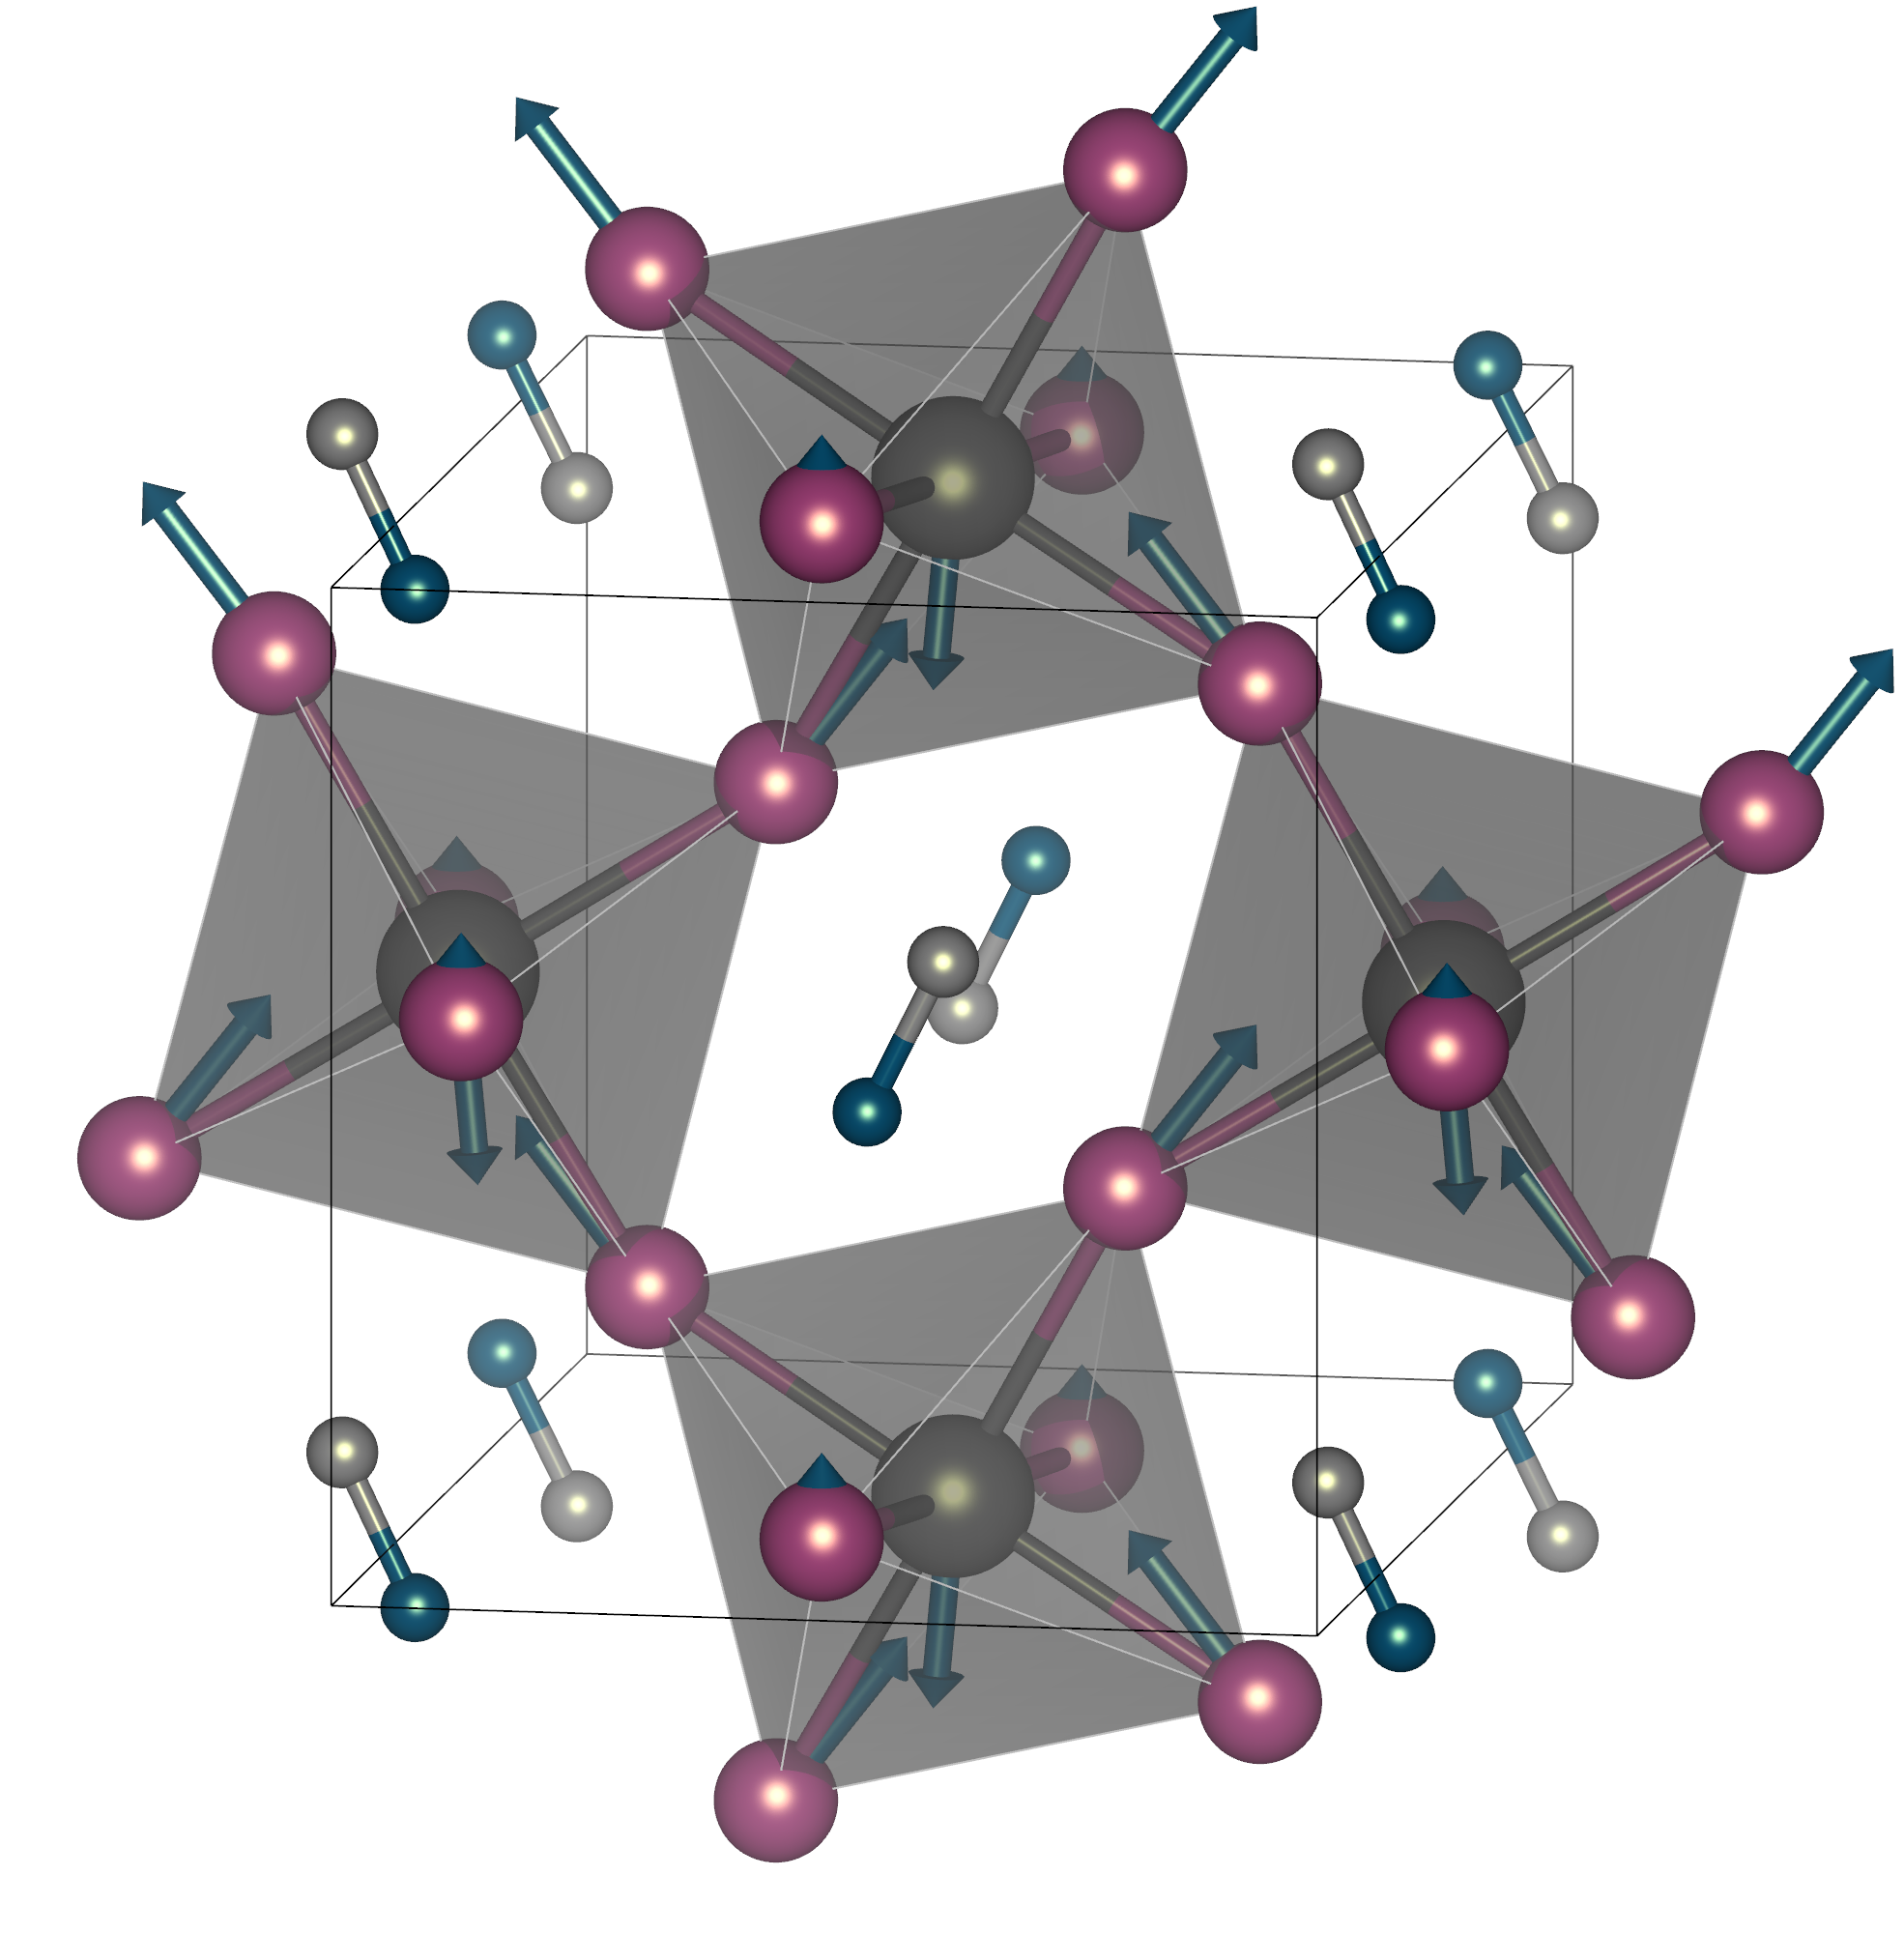
\includegraphics[width=2.7cm]{mode_two_GX-trans.png}};
    \node[] (three) at (5.6,0) {\includegraphics[width=2.7cm]{mode_three_GX-trans.png}};
  \end{scope}
  \node[below right, inner sep = 0pt] at ($(tl) - (1,-0.1)$) {(a)};
  \node[below right] at (one.north west) {(b)};
  \node at (one.south) {bending};
  \node[below right] at (two.north west) {(c)};
  \node at (two.south) {stretching};
  \node[below right] at (three.north west) {(d)};
  \node at (three.south) {libr.-trans.};
\end{tikzpicture}
\endpgfgraphicnamed
\caption{\blindtext}
\end{figure}

\begin{figure*}
  \beginpgfgraphicnamed{self_energy}%
  \begin{tikzpicture}%
    \begin{groupplot}[
      group style = {
        group size = 3 by 2,
        horizontal sep = 10pt,
        vertical sep = 10pt,
        x descriptions at=edge bottom,
        y descriptions at=edge left,
      },
      width = 0.36\textwidth,
      xmin = 0, xmax = 0.5,
      xtick = {0, 0.5},
      ymin = 0, ymax = 50,
      ylabel near ticks,
    ]
    \nextgroupplot[
        ylabel = {$\text{Im}(\Sigma_{\text{v}})\thinspace(\text{meV})$},
      ]
      \addplot[altblack] table[y expr={\htrToMeV * \thisrowno{2}}]
        {data/parabolic/GX_vb_040.dat};
      \addplot[altgreen, dashed] table[y expr={\htrToMeV * \thisrowno{2}}]
        {data/gw/GX_vb_130.dat};
      \addplot[altblue, mark=*] table[y expr={\htrToMeV * \thisrowno{2}}]
        {data/epw_all_28424_5meV/data_gx_36_\point.dat};
    \nextgroupplot
      \addplot[altblack] table[y expr={\htrToMeV * \thisrowno{2}}]
        {data/parabolic/GY_vb_040.dat};
      \addplot[altgreen, dashed] table[y expr={\htrToMeV * \thisrowno{2}}]
        {data/gw/GY_vb_130.dat};
      \addplot[altblue, mark=*] table[y expr={\htrToMeV * \thisrowno{2}}]
        {data/epw_all_28424_5meV/data_gy_36_\point.dat};
    \nextgroupplot
      \addplot[altblack] table[y expr={\htrToMeV * \thisrowno{2}}]
        {data/parabolic/GZ_vb_040.dat};
      \addplot[altgreen, dashed] table[y expr={\htrToMeV * \thisrowno{2}}]
        {data/gw/GZ_vb_130.dat};
      \addplot[altblue, mark=*] table[y expr={\htrToMeV * \thisrowno{2}}]
        {data/epw_all_28424_5meV/data_gz_36_\point.dat};
    \nextgroupplot[
        xticklabels = {$\Gamma$, X},
        ylabel = {$\text{Im}(\Sigma_{\text{c}})\thinspace(\text{meV})$},
      ]
      \addplot[altblack] table[y expr={\htrToMeV * \thisrowno{2}}]
        {data/parabolic/GX_cb_040.dat};
      \addplot[altgreen, dashed] table[y expr={\htrToMeV * \thisrowno{2}}]
        {data/gw/GX_cb_130.dat};
      \addplot[altblue, mark=*] table[y expr={\htrToMeV * \thisrowno{2}}]
        {data/epw_all_28424_5meV/data_gx_37_\point.dat};
    \nextgroupplot[
        xticklabels = {$\Gamma$, Y},
      ]
      \addplot[altblack] table[y expr={\htrToMeV * \thisrowno{2}}]
        {data/parabolic/GY_cb_040.dat};
      \addplot[altgreen, dashed] table[y expr={\htrToMeV * \thisrowno{2}}]
        {data/gw/GY_cb_130.dat};
      \addplot[altblue, mark=*] table[y expr={\htrToMeV * \thisrowno{2}}]
        {data/epw_all_28424_5meV/data_gy_37_\point.dat};
    \nextgroupplot[
        xticklabels = {$\Gamma$, Z},
      ]
      \addplot[altblack] table[y expr={\htrToMeV * \thisrowno{2}}]
        {data/parabolic/GZ_cb_040.dat};
      \addplot[altgreen, dashed] table[y expr={\htrToMeV * \thisrowno{2}}]
        {data/gw/GZ_cb_130.dat};
      \addplot[altblue, mark=*] table[y expr={\htrToMeV * \thisrowno{2}}]
        {data/epw_all_28424_5meV/data_gz_37_\point.dat};
    \end{groupplot}
  \end{tikzpicture}%
  \endpgfgraphicnamed
  \caption{\blindtext}
\end{figure*}

\begin{figure}
  \beginpgfgraphicnamed{real_part}%
  \begin{tikzpicture}%
    \begin{axis}[
      width = \columnwidth, height = 0.6\columnwidth,
      xmin = 0, xmax = 0.5,
      xtick = {0, 0.5},
      xticklabels = {$\Gamma$, X},
      ymin = -35, ymax = 0,
      ylabel = {$\text{Re}(\Sigma_{\text{c}})\thinspace(\text{meV})$},
      ylabel near ticks,
    ]
      \addplot[altblack] table[y expr={\htrToMeV * \rePart}]
        {data/symmetrized/GX_cb_030.dat};
      \addplot[altgreen, dashed] table[y expr={\htrToMeV * \rePart}]
        {data/gw/GX_cb_030.dat};
      \addplot[altblue, mark=diamond*] table[y expr={\htrToMeV * \rePart}]
        {data/epw_all_28424_1meV/data_gx_37_\point.dat};
      \addplot[altblue, mark=*] table[y expr={\htrToMeV * \rePart}]
        {data/epw_all_28424_5meV/data_gx_37_\point.dat};
    \end{axis}
  \end{tikzpicture}%
  \endpgfgraphicnamed
\end{figure}


\begin{figure}
  \beginpgfgraphicnamed{temp_dep}%
  \begin{tikzpicture}%
    \begin{axis}[
      width = \columnwidth, height = \columnwidth,
      xmin = 0, xmax = 0.5,
      xtick = {0, 0.5},
      xticklabels = {$\Gamma$, X},
      ymin = 0, ymax = 100,
      ylabel = {$\text{Im}(\Sigma_{\text{c}})\thinspace(\text{meV})$},
      ylabel near ticks,
    ]
      \addplot[altblack] table[y expr={\htrToMeV * \thisrowno{2}}]
        {data/parabolic/GX_cb_040.dat};
      \addplot[altblack] table[y expr={\htrToMeV * \thisrowno{2}}]
        {data/parabolic/GX_cb_041.dat};
      \addplot[altblack] table[y expr={\htrToMeV * \thisrowno{2}}]
        {data/parabolic/GX_cb_042.dat};
      \addplot[altblack] table[y expr={\htrToMeV * \thisrowno{2}}]
        {data/parabolic/GX_cb_043.dat};
      \addplot[altblack] table[y expr={\htrToMeV * \thisrowno{2}}]
        {data/parabolic/GX_cb_044.dat};
      \addplot[altblack] table[y expr={\htrToMeV * \thisrowno{2}}]
        {data/parabolic/GX_cb_045.dat};
      \addplot[altblack] table[y expr={\htrToMeV * \thisrowno{2}}]
        {data/parabolic/GX_cb_046.dat};
      \addplot[altblue, mark=*] table[y expr={\htrToMeV * \thisrowno{2}}]
        {data/epw_all_28424_5meV/data_gx_37_\point.dat};
      \addplot[altblue, mark=diamond*] table[y expr={\htrToMeV * \thisrowno{2}}]
        {data/epw_all_28424_50K_5meV/data_gx_37_\point.dat};
      \addplot[altblue, mark=triangle*] table[y expr={\htrToMeV * \thisrowno{2}}]
        {data/epw_all_28424_150K_5meV/data_gx_37_\point.dat};
      \node[below left] at (axis cs:0.5, 23.1089) {\footnotesize $1\thinspace\text{K}$};
      \node[above left] at (axis cs:0.5, 25.4578) {\footnotesize $50\thinspace\text{K}$};
      \node[above left] at (axis cs:0.5, 34.2445) {\footnotesize $100\thinspace\text{K}$};
      \node[above left] at (axis cs:0.5, 45.6674) {\footnotesize $150\thinspace\text{K}$};
      \node[above left] at (axis cs:0.5, 57.9741) {\footnotesize $200\thinspace\text{K}$};
      \node[above left] at (axis cs:0.5, 70.7942) {\footnotesize $250\thinspace\text{K}$};
      \node[above left] at (axis cs:0.5, 83.6831) {\footnotesize $300\thinspace\text{K}$};
    \end{axis}
  \end{tikzpicture}%
  \endpgfgraphicnamed
\end{figure}

%\begin{figure}
%  \beginpgfgraphicnamed{temp_real}%
%  \begin{tikzpicture}%
%    \begin{axis}[
%      width = \columnwidth, height = \columnwidth,
%      xmin = 0, xmax = 0.5,
%      xtick = {0, 0.5},
%      xticklabels = {$\Gamma$, X},
%%      ymin = 0, ymax = 100,
%      ylabel = {$\text{Im}(\Sigma_{\text{c}})\thinspace(\text{meV})$},
%      ylabel near ticks,
%    ]
%      \addplot[altblack] table[y expr={\htrToMeV * \rePart}]
%        {data/symmetrized/GX_cb_020.dat};
%      \addplot[altgreen] table[y expr={\htrToMeV * \rePart}]
%        {data/symmetrized/GX_cb_021.dat};
%      \addplot[altblack] table[y expr={\htrToMeV * \rePart}]
%        {data/symmetrized/GX_cb_022.dat};
%      \addplot[altyellow] table[y expr={\htrToMeV * \rePart}]
%        {data/symmetrized/GX_cb_023.dat};
%      \addplot[altblack, dashed] table[y expr={\htrToMeV * \rePart}]
%        {data/gw/GX_cb_120.dat};
%      \addplot[altgreen, dashed] table[y expr={\htrToMeV * \rePart}]
%        {data/gw/GX_cb_121.dat};
%      \addplot[altblack, dashed] table[y expr={\htrToMeV * \rePart}]
%        {data/gw/GX_cb_122.dat};
%      \addplot[altyellow, dashed] table[y expr={\htrToMeV * \rePart}]
%        {data/gw/GX_cb_123.dat};
%      \addplot[altblue, mark=*] table[y expr={\htrToMeV * \rePart}]
%        {data/epw_all_28424_5meV/data_gx_37_\point.dat};
%      \addplot[altblue, mark=diamond*] table[y expr={\htrToMeV * \rePart}]
%        {data/epw_all_28424_50K_5meV/data_gx_37_\point.dat};
%      \addplot[altblue, mark=triangle*] table[y expr={\htrToMeV * \rePart}]
%        {data/epw_all_28424_150K_5meV/data_gx_37_\point.dat};
%      \node[below left] at (axis cs:0.5, 23.1089) {\footnotesize $1\thinspace\text{K}$};
%      \node[above left] at (axis cs:0.5, 25.4578) {\footnotesize $50\thinspace\text{K}$};
%      \node[above left] at (axis cs:0.5, 34.2445) {\footnotesize $100\thinspace\text{K}$};
%      \node[above left] at (axis cs:0.5, 45.6674) {\footnotesize $150\thinspace\text{K}$};
%      \node[above left] at (axis cs:0.5, 57.9741) {\footnotesize $200\thinspace\text{K}$};
%      \node[above left] at (axis cs:0.5, 70.7942) {\footnotesize $250\thinspace\text{K}$};
%      \node[above left] at (axis cs:0.5, 83.6831) {\footnotesize $300\thinspace\text{K}$};
%    \end{axis}
%  \end{tikzpicture}%
%  \endpgfgraphicnamed
%\end{figure}

\begin{figure}
%  \begin{tikzpicture}
%    \begin{groupplot}[
%        group style = {
%          group size = 2 by 1,
%          horizontal sep = 2pt,
%          x descriptions at=edge bottom,
%          y descriptions at=edge left,
%        },
%        height = 0.7\columnwidth,
%        ymin = 0, ymax = 30,
%        ylabel = {$\text{Im}(\Sigma_{n\vect k})\thinspace(\text{meV})$},
%        ylabel near ticks,
%        scale only axis,
%      ]
%      \nextgroupplot[
%        width = 0.306\columnwidth,
%        xmin = -0.55, xmax = -0.21,
%        xtick = {-0.5, -0.3},
%        axis y line* = left,
%      ]
%      \addplot[altblack] table[
%        x expr={\htrToEV * (\thisrowno{1} - \modelFermi)},
%        y expr={\htrToMeV * \thisrowno{2}}]
%        {data/parabolic/GX_vb_040.dat};
%      \addplot[altblue, mark=text, text mark={\sffamily \tiny X}] table[
%        x expr={\htrToEV * (\thisrowno{1} - \epwFermi)},
%        y expr={\htrToMeV * \thisrowno{2}}]
%        {data/epw_all_28424_5meV/data_gx_36_\point.dat};
%      \addplot[altblue, mark=text, text mark={\sffamily \tiny Y}] table[
%        x expr={\htrToEV * (\thisrowno{1} - \epwFermi)},
%        y expr={\htrToMeV * \thisrowno{2}}]
%        {data/epw_all_28424_5meV/data_gy_36_\point.dat};
%      \addplot[altblue, mark=text, text mark={\sffamily \tiny Z}] table[
%        x expr={\htrToEV * (\thisrowno{1} - \epwFermi)},
%        y expr={\htrToMeV * \thisrowno{2}}]
%        {data/epw_all_28424_5meV/data_gz_36_\point.dat};
%      \draw[thick] (rel axis cs:0.995,0) -- (rel axis cs:0.995,0.02);
%      \draw[thick] (rel axis cs:0.995,1) -- (rel axis cs:0.995,0.98);
%      \coordinate (bl) at (rel axis cs:0,0);
%      \coordinate (zl) at (axis cs:-0.3,0);
%      
%      \nextgroupplot[
%        width = 0.531\columnwidth,
%        xmin = 0.21, xmax = 0.8,
%        xtick = {0.3, 0.5, 0.7},
%        axis y line* = right,
%      ]
%      \addplot[altblack] table[
%        x expr={\htrToEV * (\thisrowno{1} - \modelFermi)},
%        y expr={\htrToMeV * \thisrowno{2}}]
%        {data/parabolic/GX_cb_040.dat};
%      \addplot[altblue, mark=text, text mark={\sffamily \tiny X}] table[
%        x expr={\htrToEV * (\thisrowno{1} - \epwFermi)},
%        y expr={\htrToMeV * \thisrowno{2}}]
%        {data/epw_all_28424_5meV/data_gx_37_\point.dat};
%      \addplot[altblue, mark=text, text mark={\sffamily \tiny Y}] table[
%        x expr={\htrToEV * (\thisrowno{1} - \epwFermi)},
%        y expr={\htrToMeV * \thisrowno{2}}]
%        {data/epw_all_28424_5meV/data_gy_37_\point.dat};
%      \addplot[altblue, mark=text, text mark={\sffamily \tiny Z}] table[
%        x expr={\htrToEV * (\thisrowno{1} - \epwFermi)},
%        y expr={\htrToMeV * \thisrowno{2}}]
%        {data/epw_all_28424_5meV/data_gz_37_\point.dat};
%      \draw[thick] (rel axis cs:0.005,0) -- (rel axis cs:0.005,0.02);
%      \draw[thick] (rel axis cs:0.005,1) -- (rel axis cs:0.005,0.98);
%      \coordinate (br) at (rel axis cs:1,0);
%      \coordinate (zr) at (axis cs:0.3,20);
%    \end{groupplot}
%    \node[below=4mm] at ($0.5*(bl) + 0.5*(br)$) {\footnotesize $\omega - E\pedex{F}\thinspace(\text{eV})$};
%    \draw[help lines] (zl) rectangle (zr);
%  \end{tikzpicture}
  \beginpgfgraphicnamed{imag-temp}%
  \begin{tikzpicture}%
    \tikzstyle{epw} = [mark size=1pt]
    \tikzstyle{model} = [densely dashed]
    \tikzstyle{GW} = [densely dotted]
    \tikzstyle{1K} = [altblue]
    \tikzstyle{50K} = [altgreen]
    \tikzstyle{100K} = [altyellow]
    \tikzstyle{150K} = [altred]
    \tikzstyle{300K} = [altblack]
    \tikzstyle{GX} = [mark=*]
    \tikzstyle{GY} = [mark=diamond*]
    \tikzstyle{GZ} = [mark=triangle*]
    \coordinate (width) at (0.05,0);
    \begin{groupplot}[
      group style = {
        group size = 1 by 2,
        vertical sep = 2pt,
        x descriptions at=edge bottom,
        y descriptions at=edge left,
      },
      width = 0.84\columnwidth, height = 0.45\columnwidth,
      xmin = -0.71186888651336301207, xmax = 0.5,
      xtick = {-0.71186888651336301207, 0, 0.5},
      xticklabels = {X, $\Gamma$, Y},
      ymin = 0, ymax = 85,
      ylabel near ticks,
      scale only axis,
    ]
    \nextgroupplot[
      ylabel = {$\text{Im}(\Sigma_{\text{v}\vect k})\thinspace(\text{meV})$},
    ]
      \addplot[model, 1K] table[
        x expr={-\bOverA * \thisrowno{0}},
        y expr={\htrToMeV * \imPart}]
        {data/parabolic/GX_vb_030_new.dat};
      \addplot[model, 50K] table[
        x expr={-\bOverA * \thisrowno{0}},
        y expr={\htrToMeV * \imPart}]
        {data/parabolic/GX_vb_031_new.dat};
      \addplot[model, 100K] table[
        x expr={-\bOverA * \thisrowno{0}},
        y expr={\htrToMeV * \imPart}]
        {data/parabolic/GX_vb_032_new.dat};
      \addplot[model, 150K] table[
        x expr={-\bOverA * \thisrowno{0}},
        y expr={\htrToMeV * \imPart}]
        {data/parabolic/GX_vb_033_new.dat};
      \addplot[model, 300K] table[
        x expr={-\bOverA * \thisrowno{0}},
        y expr={\htrToMeV * \imPart}]
        {data/parabolic/GX_vb_036_new.dat};
      \addplot[model, 1K] table[y expr={\htrToMeV * \imPart}]
        {data/parabolic/GY_vb_040.dat};
      \addplot[model, 50K] table[y expr={\htrToMeV * \imPart}]
        {data/parabolic/GY_vb_041.dat};
      \addplot[model, 100K] table[y expr={\htrToMeV * \imPart}]
        {data/parabolic/GY_vb_042.dat};
      \addplot[model, 150K] table[y expr={\htrToMeV * \imPart}]
        {data/parabolic/GY_vb_043.dat};
      \addplot[epw, 1K, GX] table[
        x expr={-\bOverA * \thisrowno{0}},
        y expr={\htrToMeV * \imPart}]
        {data/epw_all_28424_5meV/data_gx_36_\point.dat};
      \addplot[epw, 50K, GX] table[
        x expr={-\bOverA * \thisrowno{0}},
        y expr={\htrToMeV * \imPart}]
        {data/epw_all_28424_50K_5meV/data_gx_36_\point.dat};
      \addplot[epw, 150K, GX] table[
        x expr={-\bOverA * \thisrowno{0}},
        y expr={\htrToMeV * \imPart}]
        {data/epw_all_28424_150K_5meV/data_gx_36_\point.dat};
      \addplot[epw, 300K, GX] table[
        x expr={-\bOverA * \thisrowno{0}},
        y expr={\htrToMeV * \imPart}]
        {data/epw_all_28424_300K_5meV/data_gx_36_6000.dat};
      \addplot[epw, 1K, GY] table[y expr={\htrToMeV * \imPart}]
        {data/epw_all_28424_5meV/data_gy_36_\point.dat};
      \addplot[epw, 50K, GY] table[y expr={\htrToMeV * \imPart}]
        {data/epw_all_28424_50K_5meV/data_gy_36_\point.dat};
      \addplot[epw, 150K, GY] table[y expr={\htrToMeV * \imPart}]
        {data/epw_all_28424_150K_5meV/data_gy_36_\point.dat};
      \coordinate (plot a) at (rel axis cs:0,1);
    
    \nextgroupplot[
      ylabel = {$\text{Im}(\Sigma_{\text{c}\vect k})\thinspace(\text{meV})$},
    ]
      \addplot[model, 1K] table[
        x expr={-\bOverA * \thisrowno{0}},
        y expr={\htrToMeV * \imPart}]
        {data/parabolic/GX_cb_040.dat};
      \addplot[model, 50K] table[
        x expr={-\bOverA * \thisrowno{0}},
        y expr={\htrToMeV * \imPart}]
        {data/parabolic/GX_cb_041.dat};
      \addplot[model, 100K] table[
        x expr={-\bOverA * \thisrowno{0}},
        y expr={\htrToMeV * \imPart}]
        {data/parabolic/GX_cb_042.dat};
      \addplot[model, 150K] table[
        x expr={-\bOverA * \thisrowno{0}},
        y expr={\htrToMeV * \imPart}]
        {data/parabolic/GX_cb_043.dat};
      \addplot[model, 1K] table[y expr={\htrToMeV * \imPart}]
        {data/parabolic/GY_cb_040.dat};
      \addplot[model, 50K] table[y expr={\htrToMeV * \imPart}]
        {data/parabolic/GY_cb_041.dat};
      \addplot[model, 100K] table[y expr={\htrToMeV * \imPart}]
        {data/parabolic/GY_cb_042.dat};
      \addplot[model, 150K] table[y expr={\htrToMeV * \imPart}]
        {data/parabolic/GY_cb_043.dat};
      \addplot[epw, 1K, GX] table[
        x expr={-\bOverA * \thisrowno{0}},
        y expr={\htrToMeV * \imPart}]
        {data/epw_all_28424_5meV/data_gx_37_\point.dat};
      \addplot[epw, 50K, GX] table[
        x expr={-\bOverA * \thisrowno{0}},
        y expr={\htrToMeV * \imPart}]
        {data/epw_all_28424_50K_5meV/data_gx_37_\point.dat};
      \addplot[epw, 150K, GX] table[
        x expr={-\bOverA * \thisrowno{0}},
        y expr={\htrToMeV * \imPart}]
        {data/epw_all_28424_150K_5meV/data_gx_37_\point.dat};
      \addplot[epw, 1K, GY] table[y expr={\htrToMeV * \imPart}]
        {data/epw_all_28424_5meV/data_gy_37_\point.dat};
      \addplot[epw, 50K, GY] table[y expr={\htrToMeV * \imPart}]
        {data/epw_all_28424_50K_5meV/data_gy_37_\point.dat};
      \addplot[epw, 150K, GY] table[y expr={\htrToMeV * \imPart}]
        {data/epw_all_28424_150K_5meV/data_gy_37_\point.dat};
      \coordinate (plot b) at (rel axis cs:0,1);
    \end{groupplot}
    \begin{scope}[shift={(0,-8.3)}]
    \begin{groupplot}[
        group style = {
          group size = 2 by 1,
          horizontal sep = 2pt,
          x descriptions at=edge bottom,
          y descriptions at=edge left,
        },
        height = 0.45\columnwidth,
        ymin = 0, ymax = 20,
        ylabel = {$\text{Im}(\Sigma_{n\vect k})\thinspace(\text{meV})$},
        ylabel near ticks,
        scale only axis,
      ]
      \nextgroupplot[
        width = 0.42\columnwidth,
        xmin = -0.41, xmax = -0.22,
        xtick = {-0.40, -0.35, -0.30, -0.25},
        axis y line* = left,
      ]
      \fill[altblue] ($(axis cs:-0.282,0.00) - (width)$) rectangle
                     ($(axis cs:-0.282,9.33) + (width)$);
      \fill[altred]  ($(axis cs:-0.282,9.33) - (width)$) rectangle
                     ($(axis cs:-0.282,9.33+4.77) + (width)$);
      \addplot[model, 1K] table[
        x expr={\htrToEV * (\thisrowno{1} - \modelFermi)},
        y expr={\htrToMeV * \imPart}]
        {data/parabolic/GX_vb_040.dat};
      \addplot[GW, 1K] table[
        x expr={\htrToEV * (\thisrowno{1} - \gwFermi + \gapCorr)},
        y expr={\htrToMeV * \imPart}]
        {data/parabolic/GX_vb_140.dat};
      \addplot[epw, 1K, GX] table[
        x expr={\htrToEV * (\thisrowno{1} - \epwFermi)},
        y expr={\htrToMeV * \imPart}]
        {data/epw_all_28424_5meV/data_gx_36_\point.dat};
      \addplot[epw, 1K, GY] table[
        x expr={\htrToEV * (\thisrowno{1} - \epwFermi)},
        y expr={\htrToMeV * \imPart}]
        {data/epw_all_28424_5meV/data_gy_36_\point.dat};
      \addplot[epw, 1K, GZ] table[
        x expr={\htrToEV * (\thisrowno{1} - \epwFermi)},
        y expr={\htrToMeV * \imPart}]
        {data/epw_all_28424_5meV/data_gz_36_\point.dat};
      \draw[thick] (rel axis cs:0.995,0) -- (rel axis cs:0.995,0.02);
      \draw[thick] (rel axis cs:0.995,1) -- (rel axis cs:0.995,0.98);
      \coordinate (bl) at (rel axis cs:0,0);
      \coordinate (plot c) at (rel axis cs:0,1);

      \nextgroupplot[
        width = 0.42\columnwidth,
        xmin = 0.22, xmax = 0.41,
        xtick = {0.25, 0.30, 0.35, 0.40},
        axis y line* = right,
      ]
      \fill[altblue] ($(axis cs:0.288,0.00) - (width)$) rectangle
                     ($(axis cs:0.288,8.84) + (width)$);
      \fill[altred]  ($(axis cs:0.288,8.84) - (width)$) rectangle
                     ($(axis cs:0.288,8.84+4.59) + (width)$);
      \addplot[model, 1K] table[
        x expr={\htrToEV * (\thisrowno{1} - \modelFermi)},
        y expr={\htrToMeV * \imPart}]
        {data/parabolic/GX_cb_040.dat};
      \addplot[GW, 1K] table[
        x expr={\htrToEV * (\thisrowno{1} - \gwFermi - \gapCorr)},
        y expr={\htrToMeV * \imPart}]
        {data/parabolic/GX_cb_140.dat};
      \addplot[epw, 1K, GX] table[
        x expr={\htrToEV * (\thisrowno{1} - \epwFermi)},
        y expr={\htrToMeV * \imPart}]
        {data/epw_all_28424_5meV/data_gx_37_\point.dat};
      \addplot[epw, 1K, GY] table[
        x expr={\htrToEV * (\thisrowno{1} - \epwFermi)},
        y expr={\htrToMeV * \imPart}]
        {data/epw_all_28424_5meV/data_gy_37_\point.dat};
      \addplot[epw, 1K, GZ] table[
        x expr={\htrToEV * (\thisrowno{1} - \epwFermi)},
        y expr={\htrToMeV * \imPart}]
        {data/epw_all_28424_5meV/data_gz_37_\point.dat};
      \draw[thick] (rel axis cs:0.005,0) -- (rel axis cs:0.005,0.02);
      \draw[thick] (rel axis cs:0.005,1) -- (rel axis cs:0.005,0.98);
      \coordinate (br) at (rel axis cs:1,0);
                     
    \end{groupplot}
    \node[below=4mm] at ($0.5*(bl) + 0.5*(br)$) {\footnotesize $\omega - E\pedex{F}\thinspace(\text{eV})$};
    \end{scope}
    \coordinate (shift) at (0.95, 0);
    \node[below right, inner sep = 0pt] at ($(plot a) - (shift)$) {(a)};
    \node[below right, inner sep = 0pt] at ($(plot b) - (shift)$) {(b)};
    \node[below right, inner sep = 0pt] at ($(plot c) - (shift)$) {(c)};
  \end{tikzpicture}%
  \endpgfgraphicnamed
\end{figure}

\begin{figure}
  \beginpgfgraphicnamed{real-temp}%
  \begin{tikzpicture}%
    \tikzstyle{epw} = [mark size=1pt]
    \tikzstyle{model} = [densely dashed]
    \tikzstyle{GW} = [densely dotted]
    \tikzstyle{1K} = [altblue]
    \tikzstyle{50K} = [altgreen]
    \tikzstyle{100K} = [altyellow]
    \tikzstyle{150K} = [altred]
    \tikzstyle{GX} = [mark=*]
    \tikzstyle{GY} = [mark=diamond*]
    \tikzstyle{GZ} = [mark=triangle*]
    \coordinate (width) at (0.05,0);
    \begin{groupplot}[
      group style = {
        group size = 1 by 2,
        vertical sep = 2pt,
        x descriptions at=edge bottom,
        y descriptions at=edge left,
      },
      width = 0.84\columnwidth + 2pt, height = 0.45\columnwidth,
      xmin = -0.71186888651336301207, xmax = 0.5,
      xtick = {-0.71186888651336301207, 0, 0.5},
      xticklabels = {X, $\Gamma$, Y},
%      xmin = -0.28474755460534520483, xmax = 0.2,
%      xtick = {-0.28474755460534520483, 0, 0.2},
%      xticklabels = {$\Sigma(u=\frac25)$, $\Gamma$, $\Delta(u=\frac25)$},
      ylabel near ticks,
      scale only axis,
    ]
    \nextgroupplot[
       ymin = -8, ymax = 24,
       ytick = {0, 10, 20},
%      ymin = -5, ymax = 15,
%      ytick = {-5, 0, 5, 10, 15},
%      yticklabels = {\llap{$-$}5, 0, 5, 10, 15},
      ylabel = {$\text{Re}(\Sigma_{\text{v}\vect k}-\Sigma_{\text{v}\vect 0})\thinspace(\text{meV})$},
    ]
      \draw[help lines] (axis cs:-1,0) -- (axis cs:1,0);
      \addplot[model, 1K] table[
        x expr={-\bOverA * \thisrowno{0}},
        y expr={\htrToMeV * (\rePart - \modelReVBa)}]
        {data/parabolic/GX_vb_020.dat};
      \addplot[model, 50K] table[
        x expr={-\bOverA * \thisrowno{0}},
        y expr={\htrToMeV * (\rePart - \modelReVBb)}]
        {data/parabolic/GX_vb_021.dat};
%      \addplot[model, 100K] table[
%        x expr={-\bOverA * \thisrowno{0}},
%        y expr={\htrToMeV * (\rePart - \modelReVBc)}]
%        {data/parabolic/GX_vb_022.dat};
      \addplot[model, 150K] table[
        x expr={-\bOverA * \thisrowno{0}},
        y expr={\htrToMeV * (\rePart - \modelReVBd)}]
        {data/parabolic/GX_vb_023.dat};
      \addplot[model, 1K] table[y expr={\htrToMeV * (\rePart - \modelReVBa)}]
        {data/parabolic/GY_vb_020.dat};
      \addplot[model, 50K] table[y expr={\htrToMeV * (\rePart - \modelReVBb)}]
        {data/parabolic/GY_vb_021.dat};
%      \addplot[model, 100K] table[y expr={\htrToMeV * (\rePart - \modelReVBc)}]
%        {data/parabolic/GY_vb_022.dat};
      \addplot[model, 150K] table[y expr={\htrToMeV * (\rePart - \modelReVBd)}]
        {data/parabolic/GY_vb_023.dat};
      \addplot[epw, 1K, GX] table[
        x expr={-\bOverA * \thisrowno{0}},
        y expr={\htrToMeV * (\rePart - \epwReVBa)}]
        {data/epw_all_28424_5meV/data_gx_36_\point.dat};
      \addplot[epw, 50K, GX] table[
        x expr={-\bOverA * \thisrowno{0}},
        y expr={\htrToMeV * (\rePart - \epwReVBb)}]
        {data/epw_all_28424_50K_5meV/data_gx_36_\point.dat};
      \addplot[epw, 150K, GX] table[
        x expr={-\bOverA * \thisrowno{0}},
        y expr={\htrToMeV * (\rePart - \epwReVBd)}]
        {data/epw_all_28424_150K_5meV/data_gx_36_\point.dat};
      \addplot[epw, 1K, GY] table[y expr={\htrToMeV * (\rePart - \epwReVBa)}]
        {data/epw_all_28424_5meV/data_gy_36_\point.dat};
      \addplot[epw, 50K, GY] table[y expr={\htrToMeV * (\rePart - \epwReVBb)}]
        {data/epw_all_28424_50K_5meV/data_gy_36_\point.dat};
      \addplot[epw, 150K, GY] table[y expr={\htrToMeV * (\rePart - \epwReVBd)}]
        {data/epw_all_28424_150K_5meV/data_gy_36_\point.dat};
      \coordinate (plot a) at (rel axis cs:0,1);
    
    \nextgroupplot[
      ymin = -24, ymax = 8,
      ytick = {-20, -10, 0},
      yticklabels = {\llap{$-$}20, \llap{$-$}10, 0},
%      ymin = -15, ymax = 5,
%      yticklabels = {\llap{$-$}15, \llap{$-$}10, \llap{$-$}5, 0, 5},
      ylabel = {$\text{Re}(\Sigma_{\text{c}\vect k}-\Sigma_{\text{c}\vect 0})\thinspace(\text{meV})$},
    ]
      \draw[help lines] (axis cs:-1,0) -- (axis cs:1,0);
      \addplot[model, 1K] table[
        x expr={-\bOverA * \thisrowno{0}},
        y expr={\htrToMeV * (\rePart - \modelReCBa)}]
        {data/parabolic/GX_cb_020.dat};
      \addplot[model, 50K] table[
        x expr={-\bOverA * \thisrowno{0}},
        y expr={\htrToMeV * (\rePart - \modelReCBb)}]
        {data/parabolic/GX_cb_021.dat};
%      \addplot[model, 100K] table[
%        x expr={-\bOverA * \thisrowno{0}},
%        y expr={\htrToMeV * (\rePart - \modelReCBc)}]
%        {data/parabolic/GX_cb_022.dat};
      \addplot[model, 150K] table[
        x expr={-\bOverA * \thisrowno{0}},
        y expr={\htrToMeV * (\rePart - \modelReCBd)}]
        {data/parabolic/GX_cb_023.dat};
      \addplot[model, 1K] table[y expr={\htrToMeV * (\rePart - \modelReCBa)}]
        {data/parabolic/GY_cb_020.dat};
      \addplot[model, 50K] table[y expr={\htrToMeV * (\rePart - \modelReCBb)}]
        {data/parabolic/GY_cb_021.dat};
%      \addplot[model, 100K] table[y expr={\htrToMeV * (\rePart - \modelReCBc)}]
%        {data/parabolic/GY_cb_022.dat};
      \addplot[model, 150K] table[y expr={\htrToMeV * (\rePart - \modelReCBd)}]
        {data/parabolic/GY_cb_023.dat};
      \addplot[epw, 1K, GX] table[
        x expr={-\bOverA * \thisrowno{0}},
        y expr={\htrToMeV * (\rePart - \epwReCBa)}]
        {data/epw_all_28424_5meV/data_gx_37_\point.dat};
      \addplot[epw, 50K, GX] table[
        x expr={-\bOverA * \thisrowno{0}},
        y expr={\htrToMeV * (\rePart - \epwReCBb)}]
        {data/epw_all_28424_50K_5meV/data_gx_37_\point.dat};
      \addplot[epw, 150K, GX] table[
        x expr={-\bOverA * \thisrowno{0}},
        y expr={\htrToMeV * (\rePart - \epwReCBd)}]
        {data/epw_all_28424_150K_5meV/data_gx_37_\point.dat};
      \addplot[epw, 1K, GY] table[y expr={\htrToMeV * (\rePart - \epwReCBa)}]
        {data/epw_all_28424_5meV/data_gy_37_\point.dat};
      \addplot[epw, 50K, GY] table[y expr={\htrToMeV * (\rePart - \epwReCBb)}]
        {data/epw_all_28424_50K_5meV/data_gy_37_\point.dat};
      \addplot[epw, 150K, GY] table[y expr={\htrToMeV * (\rePart - \epwReCBd)}]
        {data/epw_all_28424_150K_5meV/data_gy_37_\point.dat};
      \coordinate (plot b) at (rel axis cs:0,1);
    \end{groupplot}
    \begin{scope}[shift={(0,-8.3)}]
    \begin{groupplot}[
        group style = {
          group size = 2 by 1,
          horizontal sep = 2pt,
          x descriptions at=edge bottom,
          y descriptions at=edge left,
        },
        height = 0.45\columnwidth,
        ymin = -6, ymax = 6,
        ytick = {-5, 0, 5},
        yticklabels = {\hphantom{2}\llap{$-$}5, 0, 5},
        ylabel = {$\text{Re}(\Sigma_{n\vect k}-\Sigma_{n\vect 0})\thinspace(\text{meV})$},
        ylabel near ticks,
        scale only axis,
      ]
      \nextgroupplot[
        width = 0.42\columnwidth,
        xmin = -0.41, xmax = -0.22,
        xtick = {-0.40, -0.35, -0.30, -0.25},
        axis y line* = left,
      ]
      \draw[help lines] (axis cs:-1,0) -- (axis cs:1,0);
      \draw[help lines] (axis cs:-\gap,0) -- (axis cs:-0.006/0.314343-\gap, 6)
        node[below left,black,inner sep=1pt] {\tiny $-0.31$};
      \fill[altblue] ($(axis cs:-0.250,0.00) - (width)$) rectangle
                     ($(axis cs:-0.250,1.699) + (width)$);
      \fill[altred]  ($(axis cs:-0.250,1.699) - (width)$) rectangle
                     ($(axis cs:-0.250,1.699+1.063) + (width)$);
      \addplot[model, 1K] table[
        x expr={\htrToEV * (\thisrowno{1} - \modelFermi)},
        y expr={\htrToMeV * (\rePart - \modelReVBa)}]
        {data/parabolic/GY_vb_020.dat};
      \addplot[GW, 1K] table[
        x expr={\htrToEV * (\thisrowno{1} - \gwFermi + \gapCorr)},
        y expr={\htrToMeV * (\rePart - \gwReVBa)}]
        {data/parabolic/GY_vb_120.dat};
      \addplot[epw, 1K, GX] table[
        x expr={\htrToEV * (\thisrowno{1} - \epwFermi)},
        y expr={\htrToMeV * (\rePart - \epwReVBa)}]
        {data/epw_all_28424_5meV/data_gx_36_\point.dat};
      \addplot[epw, 1K, GY] table[
        x expr={\htrToEV * (\thisrowno{1} - \epwFermi)},
        y expr={\htrToMeV * (\rePart - \epwReVBa)}]
        {data/epw_all_28424_5meV/data_gy_36_\point.dat};
      \addplot[epw, 1K, GZ] table[
        x expr={\htrToEV * (\thisrowno{1} - \epwFermi)},
        y expr={\htrToMeV * (\rePart - \epwReVBa)}]
        {data/epw_all_28424_5meV/data_gz_36_\point.dat};
      \draw[thick] (rel axis cs:0.995,0) -- (rel axis cs:0.995,0.02);
      \draw[thick] (rel axis cs:0.995,1) -- (rel axis cs:0.995,0.98);
      \coordinate (bl) at (rel axis cs:0,0);
      \coordinate (plot c) at (rel axis cs:0,1);
      
      \nextgroupplot[
        width = 0.42\columnwidth,
        xmin = 0.22, xmax = 0.41,
        xtick = {0.25, 0.30, 0.35, 0.40},
        axis y line* = right,
      ]
      \draw[help lines] (axis cs:-1,0) -- (axis cs:1,0);
      \draw[help lines] (axis cs:\gap,0) -- (axis cs:0.006/0.26234+\gap, -6)
        node[above right,black,inner sep=1pt] {\tiny $-0.26$};
      \fill[altblue] ($(axis cs:0.253, 0.000) - (width)$) rectangle
                     ($(axis cs:0.253,-1.664) + (width)$);
      \fill[altred]  ($(axis cs:0.253,-1.664) - (width)$) rectangle
                     ($(axis cs:0.253,-1.664-0.968) + (width)$);
      \addplot[model, 1K] table[
        x expr={\htrToEV * (\thisrowno{1} - \modelFermi)},
        y expr={\htrToMeV * (\rePart - \modelReCBa)}]
        {data/parabolic/GY_cb_020.dat};
      \addplot[GW, 1K] table[
        x expr={\htrToEV * (\thisrowno{1} - \gwFermi - \gapCorr)},
        y expr={\htrToMeV * (\rePart - \gwReCBa)}]
        {data/parabolic/GY_cb_120.dat};
      \addplot[epw, 1K, GX] table[
        x expr={\htrToEV * (\thisrowno{1} - \epwFermi)},
        y expr={\htrToMeV * (\rePart - \epwReCBa)}]
        {data/epw_all_28424_5meV/data_gx_37_\point.dat};
      \addplot[epw, 1K, GY] table[
        x expr={\htrToEV * (\thisrowno{1} - \epwFermi)},
        y expr={\htrToMeV * (\rePart - \epwReCBa)}]
        {data/epw_all_28424_5meV/data_gy_37_\point.dat};
      \addplot[epw, 1K, GZ] table[
        x expr={\htrToEV * (\thisrowno{1} - \epwFermi)},
        y expr={\htrToMeV * (\rePart - \epwReCBa)}]
        {data/epw_all_28424_5meV/data_gz_37_\point.dat};
      \draw[thick] (rel axis cs:0.005,0) -- (rel axis cs:0.005,0.02);
      \draw[thick] (rel axis cs:0.005,1) -- (rel axis cs:0.005,0.98);
      \coordinate (br) at (rel axis cs:1,0);
    \end{groupplot}
    \node[below=4mm] at ($0.5*(bl) + 0.5*(br)$) {\footnotesize $\omega - E\pedex{F}\thinspace(\text{eV})$};
    \end{scope}
    \coordinate (shift) at (0.95, 0);
    \node[below right, inner sep = 0pt] at ($(plot a) - (shift)$) {(a)};
    \node[below right, inner sep = 0pt] at ($(plot b) - (shift)$) {(b)};
    \node[below right, inner sep = 0pt] at ($(plot c) - (shift)$) {(c)};
  \end{tikzpicture}%
  \endpgfgraphicnamed
\end{figure}

\begin{figure}
  \beginpgfgraphicnamed{physical}%
  \begin{tikzpicture}%
    \tikzstyle{epw} = [only marks,mark size=1.5pt]
    \tikzstyle{model} = [altgreen]
    \tikzstyle{RS} = [dashed]
    \tikzstyle{BW} = []
    \tikzstyle{expt} = [only marks,mark=square*,fill=white]
    \tikzstyle{below step} = [mark=*]
    \tikzstyle{above step} = [mark=triangle*]
    \tikzstyle{acoustic} = [altred]
    \coordinate (width) at (0.05,0);
    \begin{scope}
    \begin{groupplot}[
        group style = {
          group size = 2 by 1,
          horizontal sep = 2pt,
          x descriptions at=edge bottom,
          y descriptions at=edge left,
        },
        height = 0.32\columnwidth,
        ymin = -0.25, ymax = 18,
        ylabel = {$\Gamma\thinspace(\text{meV})$},
        xlabel near ticks, ylabel near ticks,
        scale only axis,
      ]
      \nextgroupplot[
        width = 0.37\columnwidth,
        xmin = -105, xmax = 5,
        xtick = {0,-25,-50,-100},
        xticklabels = {0, $-\epsilon\pedex{t}$, $-50$, $-100$},
        xlabel = {$\epsilon - \epsilon\pedex{v}$~(meV)},
        axis y line* = left,
        %legend columns=3,
        legend pos=south west,
      ]
        \draw[help lines] (axis cs:-105,0) -- (axis cs:0,0);
        \fill[altyellow] ($(axis cs:-50.5,0.0) - (width)$) rectangle
                         ($(axis cs:-50.5,0.0+0.50) + (width)$);
        \fill[altblue]   ($(axis cs:-50.5,0.0+0.50) - (width)$) rectangle
                         ($(axis cs:-50.5,0.0+0.50+8.57) + (width)$);
        \fill[altred]    ($(axis cs:-50.5,0.0+0.50+8.57) - (width)$) rectangle
                         ($(axis cs:-50.5,0.0+0.50+8.57+4.59) + (width)$);
        \addplot[epw, below step, acoustic] file {data/new_model/epw_step_vb_below_acoustic.dat};
        \addplot[epw, above step, acoustic] file {data/new_model/epw_step_vb_above_acoustic.dat};
        \addplot[model, RS] file {data/new_model/step_vb_RS.dat};
        \addplot[model, BW] file {data/new_model/step_vb_BW.dat};
        \addplot[epw, below step] file {data/new_model/epw_step_vb_below.dat};
        \addplot[epw, above step] file {data/new_model/epw_step_vb_above.dat};
      \draw[thick] (rel axis cs:0.995,0) -- (rel axis cs:0.995,0.02);
      \draw[thick] (rel axis cs:0.995,1) -- (rel axis cs:0.995,0.98);
      \draw[help lines,densely dotted] (axis cs:-25,0) -- (axis cs:-25,30);
      \coordinate (bl) at (rel axis cs:0,0);
      \coordinate (plot a) at (rel axis cs:0,1);

      \nextgroupplot[
        width = 0.37\columnwidth,
        xmin = -5, xmax = 105,
        xtick = {0,25,50,100},
        xticklabels = {0, $\vphantom{-}\epsilon\pedex{t}$, $\vphantom{-}50$, $\vphantom{-}100$},
        xlabel = {$\epsilon - \epsilon\pedex{c}$~(meV)},
        axis y line* = right,
      ]
        \draw[help lines] (axis cs:0,0) -- (axis cs:105,0);
        \fill[altyellow] ($(axis cs:50.5,0.0) - (width)$) rectangle
                         ($(axis cs:50.5,0.0+0.47) + (width)$);
        \fill[altblue]   ($(axis cs:50.5,0.0+0.47) - (width)$) rectangle
                         ($(axis cs:50.5,0.0+0.47+8.18) + (width)$);
        \fill[altred]    ($(axis cs:50.5,0.0+0.47+8.18) - (width)$) rectangle
                         ($(axis cs:50.5,0.0+0.47+8.18+4.38) + (width)$);
        \addplot[epw, below step, acoustic] file {data/new_model/epw_step_cb_below_acoustic.dat};
        \addplot[epw, above step, acoustic] file {data/new_model/epw_step_cb_above_acoustic.dat};
        \addplot[model, RS] file {data/new_model/step_cb_RS.dat};
        \addplot[model, BW] file {data/new_model/step_cb_BW.dat};
        \addplot[epw, below step] file {data/new_model/epw_step_cb_below.dat};
        \addplot[epw, above step] file {data/new_model/epw_step_cb_above.dat};
      \draw[thick] (rel axis cs:0.005,0) -- (rel axis cs:0.005,0.02);
      \draw[thick] (rel axis cs:0.005,1) -- (rel axis cs:0.005,0.98);
      \draw[help lines,densely dotted] (axis cs:25,0) -- (axis cs:25,30);
      \coordinate (br) at (rel axis cs:1,0);
                     
    \end{groupplot}
    \end{scope}
    \begin{scope}[shift={(0,-4)}]
      \begin{axis}[
        width = 0.75 \columnwidth,
        height = 0.35\columnwidth,
        xmin = 0, xmax = 310,
        xticklabels = \empty,        
        ymin = -5, ymax = 260,
        ytick = {0,50,...,250},
        ylabel = {$1/\tau$\thinspace(THz)},
        ylabel near ticks,
        axis y line*=left,
        scale only axis,
        legend pos = north west,
        legend columns = 2, transpose legend,
      ]
        \draw[help lines] (axis cs:0,0) -- (axis cs:310,0);
        \fill[altyellow] ($(axis cs:300,0.0) - 3.5*(width)$) rectangle
                         ($(axis cs:300,9.16) - 1.5*(width)$);
        \fill[altblue]   ($(axis cs:300,0.0) - (width)$) rectangle
                         ($(axis cs:300,26.46) + (width)$);
        \fill[altred]    ($(axis cs:300,0.0) + 1.5*(width)$) rectangle
                         ($(axis cs:300,13.31) + 3.5*(width)$);
        \addplot[model, RS] table[y expr={0.5 * (\thisrowno{1} + \thisrowno{5})}] {data/new_model/lifetime_RS.dat};
        \addplot[model, BW] table[y expr={0.5 * (\thisrowno{1} + \thisrowno{5})}] {data/new_model/lifetime_BW.dat};
        \addplot[epw, below step] table[y index=1] {data/new_model/epw_lifetime_vb.dat};
        \addplot[epw, above step] table[y index=2] {data/new_model/epw_lifetime_vb.dat};
        \addplot[epw, below step, forget plot] table[y index=1] {data/new_model/epw_lifetime_cb.dat};
        \addplot[epw, above step, forget plot] table[y index=2] {data/new_model/epw_lifetime_cb.dat};
        \addplot[epw, above step, acoustic, forget plot] table[y index=2] {data/new_model/epw_lifetime_vb_acoustic.dat};
        \addplot[expt] table[y expr={(0.5 * \meVToTHz * \thisrowno{1}}] {data/MAPI.dat};
        \addplot[expt, mark=diamond*] table[y expr={(1000.0 / \thisrowno{1}}] {data/scatt_exp.dat};
        \coordinate (plot b) at (rel axis cs:0,1);
        \legend{model\pedex{\rlap{RS}\hphantom{BW}}, model\pedex{BW}, EPW$_{\abs\epsilon < \epsilon\pedex{t}}$, EPW$_{\abs\epsilon > \epsilon\pedex{t}}$, Ref.~19, Ref.~35}
      \end{axis}
      \begin{axis}[
        width = 0.75\columnwidth,
        height = 0.35\columnwidth,
        xmin = 0, xmax = 310,
        xlabel = {$T$\thinspace(K)},
        xlabel near ticks,
        axis x line=none,
        ymin = -0.005, ymax = 0.26,
        ytick = {0.2,0.1,0.02},
        yticklabels = {5, 10, 50},
        minor ytick = {0.25, 0.2, 0.1667, 0.1429, 0.125, 0.1111, 0.05, 0.0333, 0.025, 0.01},
        ylabel = {$\tau$\thinspace(fs)},
        ylabel near ticks,
        axis y line*=right,
        scale only axis,
        legend pos = north west,
      ]
      \end{axis}
    \end{scope}
    \begin{scope}[shift={(0,-7.05)}]
      \begin{axis}[
        width = 0.75 \columnwidth,
        height = 0.35\columnwidth,
        xmin = 0, xmax = 310,
        xlabel = {$T$\thinspace(K)},
        xlabel near ticks,
        ymin = -0.01, ymax = 0.68,
        ylabel = {$\lambda$},
        ylabel near ticks,
        scale only axis,
        legend pos = north west,
      ]
        \draw[help lines] (axis cs:0,0) -- (axis cs:310,0);
        \fill[altyellow] ($(axis cs:1,0.0)$) rectangle
                         ($(axis cs:1,0.034) + 2*(width)$);
        \fill[altblue]   ($(axis cs:1,0.0) + 2.5*(width)$) rectangle
                         ($(axis cs:1,0.110) + 4.5*(width)$);
        \fill[altred]    ($(axis cs:1,0.0) + 5*(width)$) rectangle
                         ($(axis cs:1,0.048) + 7*(width)$);
        \fill[altyellow] ($(axis cs:300,0.0) - 3.5*(width)$) rectangle
                         ($(axis cs:300,0.150) - 1.5*(width)$);
        \fill[altblue]   ($(axis cs:300,0.0) - (width)$) rectangle
                         ($(axis cs:300,0.185) + (width)$);
        \fill[altred]    ($(axis cs:300,0.0) + 1.5*(width)$) rectangle
                         ($(axis cs:300,0.079) + 3.5*(width)$);
        \addplot[model, RS] table[y expr={0.5 * (\thisrowno{1} + \thisrowno{4}}] {data/new_model/mass_RS.dat};
        \addplot[model, BW] table[y expr={0.5 * (\thisrowno{1} + \thisrowno{4}}] {data/new_model/mass_BW.dat};
        \addplot[epw,below step,error bars/.cd,y dir=both,y explicit] table[y index=1, y error index=2] {data/new_model/epw_mass_vb.dat};
        \addplot[epw,below step,error bars/.cd,y dir=both,y explicit] table[y index=1, y error index=2] {data/new_model/epw_mass_cb.dat};
        \addplot[epw,acoustic,below step,error bars/.cd,y dir=both,y explicit] table[y index=1, y error index=2] {data/new_model/epw_mass_vb_acoustic.dat};
        \coordinate (plot c) at (rel axis cs:0,1);
      \end{axis}
    \end{scope}
    \coordinate (shift) at (1.1, -0.1);
    \node[below right, inner sep = 0pt] at ($(plot a) - (shift)$) {(a)};
    \node[below right, inner sep = 0pt] at ($(plot b) - (shift)$) {(b)};
    \node[below right, inner sep = 0pt] at ($(plot c) - (shift)$) {(c)};
  \end{tikzpicture}%
  \endpgfgraphicnamed
  %\caption{\blindtext}
\end{figure}

\begin{figure}
  \beginpgfgraphicnamed{physical-alt}%
  \begin{tikzpicture}%
    \tikzstyle{epw} = [only marks,mark size=1.5pt]
    \tikzstyle{model} = [altgreen]
    \tikzstyle{RS} = [dashed]
    \tikzstyle{BW} = []
    \tikzstyle{expt} = [only marks,mark=square*,fill=white,mark size=1.5pt]
    \tikzstyle{below vb} = [mark=halfcircle*, mark options={rotate=180}]
    \tikzstyle{above vb} = [mark=halfsquare*]
    \tikzstyle{below cb} = [mark=halfcircle*]
    \tikzstyle{above cb} = [mark=halfsquare*, mark options={rotate=180}]
    \tikzstyle{acoustic} = [altred]
    \coordinate (width) at (0.05,0);
    \begin{scope}
    \begin{groupplot}[
        group style = {
          group size = 2 by 1,
          horizontal sep = 2pt,
          x descriptions at=edge bottom,
          y descriptions at=edge left,
        },
        height = 0.32\columnwidth,
        ymin = -0.25, ymax = 18,
        ylabel = {$\Gamma\thinspace(\text{meV})$},
        xlabel near ticks, ylabel near ticks,
        scale only axis,
      ]
      \nextgroupplot[
        width = 0.345\columnwidth,
        xmin = -110, xmax = 5,
        xtick = {0,-25,-50,-100},
        xticklabels = {0, $-\epsilon\pedex{t}$, $-50$, $-100$},
        xlabel = {$\epsilon - \epsilon\pedex{v}$~(meV)},
        axis y line* = left,
      ]
        \draw[help lines] (axis cs:-105,0) -- (axis cs:0,0);
        \fill[altyellow] ($(axis cs:-50.5,0.0) - (width)$) rectangle
                         ($(axis cs:-50.5,0.0+0.50) + (width)$);
        \fill[altblue]   ($(axis cs:-50.5,0.0+0.50) - (width)$) rectangle
                         ($(axis cs:-50.5,0.0+0.50+8.57) + (width)$);
        \fill[altred]    ($(axis cs:-50.5,0.0+0.50+8.57) - (width)$) rectangle
                         ($(axis cs:-50.5,0.0+0.50+8.57+4.59) + (width)$);
        \addplot[epw, below vb, acoustic] file {data/new_model/epw_step_vb_below_acoustic.dat};
        \addplot[epw, above vb, acoustic] file {data/new_model/epw_step_vb_above_acoustic.dat};
        \addplot[model, RS] file {data/new_model/step_vb_RS.dat};
        \addplot[model, BW] file {data/new_model/step_vb_BW.dat};
        \addplot[epw, below vb] file {data/new_model/epw_step_vb_below.dat};
        \addplot[epw, above vb] file {data/new_model/epw_step_vb_above.dat};
      \draw[thick] (rel axis cs:0.995,0) -- (rel axis cs:0.995,0.02);
      \draw[thick] (rel axis cs:0.995,1) -- (rel axis cs:0.995,0.98);
      \draw[help lines,densely dotted] (axis cs:-25,0) -- (axis cs:-25,30);
      \coordinate (bl) at (rel axis cs:0,0);
      \coordinate (plot a) at (rel axis cs:0,1);

      \nextgroupplot[
        width = 0.345\columnwidth,
        xmin = -5, xmax = 110,
        xtick = {0,25,50,100},
        xticklabels = {0, $\vphantom{-}\epsilon\pedex{t}$, $\vphantom{-}50$, $\vphantom{-}100$},
        xlabel = {$\epsilon - \epsilon\pedex{c}$~(meV)},
        axis y line* = right,
      ]
        \draw[help lines] (axis cs:0,0) -- (axis cs:105,0);
        \fill[altyellow] ($(axis cs:50.5,0.0) - (width)$) rectangle
                         ($(axis cs:50.5,0.0+0.47) + (width)$);
        \fill[altblue]   ($(axis cs:50.5,0.0+0.47) - (width)$) rectangle
                         ($(axis cs:50.5,0.0+0.47+8.18) + (width)$);
        \fill[altred]    ($(axis cs:50.5,0.0+0.47+8.18) - (width)$) rectangle
                         ($(axis cs:50.5,0.0+0.47+8.18+4.38) + (width)$);
        \addplot[epw, below cb, acoustic] file {data/new_model/epw_step_cb_below_acoustic.dat};
        \addplot[epw, above cb, acoustic] file {data/new_model/epw_step_cb_above_acoustic.dat};
        \addplot[model, RS] file {data/new_model/step_cb_RS.dat};
        \addplot[model, BW] file {data/new_model/step_cb_BW.dat};
        \addplot[epw, below cb] file {data/new_model/epw_step_cb_below.dat};
        \addplot[epw, above cb] file {data/new_model/epw_step_cb_above.dat};
      \draw[thick] (rel axis cs:0.005,0) -- (rel axis cs:0.005,0.02);
      \draw[thick] (rel axis cs:0.005,1) -- (rel axis cs:0.005,0.98);
      \draw[help lines,densely dotted] (axis cs:25,0) -- (axis cs:25,30);
      \coordinate (br) at (rel axis cs:1,0);
      \coordinate (legend) at (rel axis cs:1,1);
                     
    \end{groupplot}
    \end{scope}
    \begin{scope}[shift={(0,-4)}]
      \begin{axis}[
        width = 0.7\columnwidth,
        height = 0.35\columnwidth,
        xmin = 0, xmax = 310,
        xticklabels = \empty,        
        ymin = -5, ymax = 260,
        ytick = {0,50,...,250},
        ylabel = {$1/\tau$\thinspace(THz)},
        ylabel near ticks,
        axis y line*=left,
        scale only axis,
      ]
        \draw[help lines] (axis cs:0,0) -- (axis cs:310,0);
        \fill[altyellow] ($(axis cs:300,0.0) - 3.5*(width)$) rectangle
                         ($(axis cs:300,9.16) - 1.5*(width)$);
        \fill[altblue]   ($(axis cs:300,0.0) - (width)$) rectangle
                         ($(axis cs:300,26.46) + (width)$);
        \fill[altred]    ($(axis cs:300,0.0) + 1.5*(width)$) rectangle
                         ($(axis cs:300,13.31) + 3.5*(width)$);
        \addplot[model, RS] table[y expr={0.5 * (\thisrowno{1} + \thisrowno{5})}] {data/new_model/lifetime_RS.dat};
        \addplot[model, BW] table[y expr={0.5 * (\thisrowno{1} + \thisrowno{5})}] {data/new_model/lifetime_BW.dat};
        \addplot[epw, below vb] table[y index=1] {data/new_model/epw_lifetime_vb.dat};
        \addplot[epw, above vb] table[y index=2] {data/new_model/epw_lifetime_vb.dat};
        \addplot[epw, below cb, forget plot] table[y index=1] {data/new_model/epw_lifetime_cb.dat};
        \addplot[epw, above cb, forget plot] table[y index=2] {data/new_model/epw_lifetime_cb.dat};
        \addplot[epw, above vb, acoustic, forget plot] table[y index=2] {data/new_model/epw_lifetime_vb_acoustic.dat};
        \addplot[expt, mark size=1.2pt] table[y expr={(0.5 * \meVToTHz * \thisrowno{1}}] {data/MAPI.dat};
        \addplot[expt, mark=triangle*] table[y expr={(1000.0 / \thisrowno{1}}] {data/scatt_exp.dat};
        \coordinate (plot b) at (rel axis cs:0,1);
      \end{axis}
      \begin{axis}[
        width = 0.7\columnwidth,
        height = 0.35\columnwidth,
        xmin = 0, xmax = 310,
        xlabel = {$T$\thinspace(K)},
        xlabel near ticks,
        axis x line=none,
        ymin = -0.005, ymax = 0.26,
        ytick = {0.2,0.1,0.02},
        yticklabels = {5, 10, 50},
        minor ytick = {0.25, 0.2, 0.1667, 0.1429, 0.125, 0.1111, 0.05, 0.0333, 0.025, 0.01},
        ylabel = {$\tau$\thinspace(fs)},
        ylabel near ticks,
        axis y line*=right,
        scale only axis,
        legend pos = north west,
      ]
      \end{axis}
    \end{scope}
    \begin{scope}[shift={(0,-7.05)}]
      \begin{axis}[
        width = 0.7\columnwidth,
        height = 0.35\columnwidth,
        xmin = 0, xmax = 310,
        xlabel = {$T$\thinspace(K)},
        xlabel near ticks,
        ymin = -0.01, ymax = 0.68,
        ylabel = {$\lambda$},
        ylabel near ticks,
        scale only axis,
        legend pos = north west,
      ]
        \draw[help lines] (axis cs:0,0) -- (axis cs:310,0);
        \fill[altyellow] ($(axis cs:1,0.0)$) rectangle
                         ($(axis cs:1,0.034) + 2*(width)$);
        \fill[altblue]   ($(axis cs:1,0.0) + 2.5*(width)$) rectangle
                         ($(axis cs:1,0.110) + 4.5*(width)$);
        \fill[altred]    ($(axis cs:1,0.0) + 5*(width)$) rectangle
                         ($(axis cs:1,0.048) + 7*(width)$);
        \fill[altyellow] ($(axis cs:300,0.0) - 3.5*(width)$) rectangle
                         ($(axis cs:300,0.150) - 1.5*(width)$);
        \fill[altblue]   ($(axis cs:300,0.0) - (width)$) rectangle
                         ($(axis cs:300,0.185) + (width)$);
        \fill[altred]    ($(axis cs:300,0.0) + 1.5*(width)$) rectangle
                         ($(axis cs:300,0.079) + 3.5*(width)$);
        \addplot[model, RS] table[y expr={0.5 * (\thisrowno{1} + \thisrowno{4}}] {data/new_model/mass_RS.dat};
        \addplot[model, BW] table[y expr={0.5 * (\thisrowno{1} + \thisrowno{4}}] {data/new_model/mass_BW.dat};
        \addplot[epw,below vb,error bars/.cd,y dir=both,y explicit] table[y index=1, y error index=2] {data/new_model/epw_mass_vb.dat};
        \addplot[epw,below cb,error bars/.cd,y dir=both,y explicit] table[y index=1, y error index=2] {data/new_model/epw_mass_cb.dat};
        \addplot[epw,acoustic,below vb,error bars/.cd,y dir=both,y explicit] table[y index=1, y error index=2] {data/new_model/epw_mass_vb_acoustic.dat};
        \coordinate (plot c) at (rel axis cs:0,1);
      \end{axis}
    \end{scope}
    \coordinate (shift) at (1.1, -0.1);
    \node[below right, inner sep = 0pt] at ($(plot a) - (shift)$) {(a)};
    \node[below right, inner sep = 0pt] at ($(plot b) - (shift)$) {(b)};
    \node[below right, inner sep = 0pt] at ($(plot c) - (shift)$) {(c)};
    \begin{scope}[shift={(legend)},scale=0.8]
      \tiny
%      \draw (0,0) grid[step = 0.1] (1.5,-5);
%      \draw[red] (0,0) grid[step = 0.5] (1.5,-5);
      \node[right] at (0.0,-0.1) {EPW};
      \draw[epw,below vb] plot coordinates {(0.2,-0.4)};
      \node[right] at (0.3,-0.4) {all, v, low};
      \draw[epw,above vb] plot coordinates {(0.2,-0.7)};
      \node[right] at (0.3,-0.7) {all, v, high};
      \draw[epw,below vb,acoustic] plot coordinates {(0.2,-1.0)};
      \node[right] at (0.3,-1.0) {ac, v, low};
      \draw[epw,above vb,acoustic] plot coordinates {(0.2,-1.3)};
      \node[right] at (0.3,-1.3) {ac, v, high};
      \draw[epw,below cb] plot coordinates {(0.2,-1.6)};
      \node[right] at (0.3,-1.6) {all, c, low};
      \draw[epw,above cb] plot coordinates {(0.2,-1.9)};
      \node[right] at (0.3,-1.9) {all, c, high};
      \draw[epw,below cb,acoustic] plot coordinates {(0.2,-2.2)};
      \node[right] at (0.3,-2.2) {ac, c, low};
      \draw[epw,above cb,acoustic] plot coordinates {(0.2,-2.5)};
      \node[right] at (0.3,-2.5) {ac, c, high};
      \node[right] at (0,-2.9) {model};
      \draw[model,RS] plot coordinates {(0.15,-3.2) (0.75,-3.2)};
      \node[right] at (0.75,-3.2) {RS};
      \draw[model,BW] plot coordinates {(0.15,-3.5) (0.75,-3.5)};
      \node[right] at (0.75,-3.5) {BW};
      \node[right] at (0,-3.9) {Expt.};
      \draw[expt, mark=triangle] plot coordinates {(0.2,-4.2)};
      \node[right] at (0.3,-4.2) {Ref.~[?]};
      \draw[expt, mark size=1.2pt] plot coordinates {(0.2,-4.5)};
      \node[right] at (0.3,-4.5) {Ref.~[?]};
    \end{scope}
  \end{tikzpicture}%
  \endpgfgraphicnamed
  \caption{\blindtext}
\end{figure}

\begin{figure}
  \beginpgfgraphicnamed{physical3}%
  \begin{tikzpicture}%
    \tikzstyle{epw} = [only marks,mark=*,mark size=1.5pt]
    \tikzstyle{model} = [altgreen]
    \tikzstyle{RS} = [dashed]
    \tikzstyle{BW} = []
    \tikzstyle{expt} = [only marks,mark=square*,fill=white,mark size=2pt]
    \tikzstyle{below} = []
    \tikzstyle{above} = [mark=diamond*,mark size=2pt]
    \tikzstyle{acoustic} = [altred]
    \coordinate (width) at (0.05,0);
    \begin{scope}
    \begin{groupplot}[
        group style = {
          group size = 2 by 1,
          horizontal sep = 2pt,
          x descriptions at=edge bottom,
          y descriptions at=edge left,
        },
        height = 0.36\columnwidth,
        ymin = -0.25, ymax = 22,
        ylabel = {$\Gamma\thinspace(\text{meV})$},
        xlabel near ticks, ylabel near ticks,
        scale only axis,
      ]
      \nextgroupplot[
        width = 0.37\columnwidth,
        xmin = -110, xmax = 5,
        xtick = {0,-25,-50,-100},
        xticklabels = {0, $-\hat\varepsilon\pedex{LO}$, $-50$, $-100$},
        xlabel = {$\varepsilon - \varepsilon\pedex{v}$~(meV)},
        axis y line* = left,
      ]
        \draw[help lines] (axis cs:-105,0) -- (axis cs:0,0);
        \fill[altyellow] ($(axis cs:-50.5,0.0) - (width)$) rectangle
                         ($(axis cs:-50.5,0.0+0.50) + (width)$);
        \fill[altblue]   ($(axis cs:-50.5,0.0+0.50) - (width)$) rectangle
                         ($(axis cs:-50.5,0.0+0.50+8.57) + (width)$);
        \fill[altred]    ($(axis cs:-50.5,0.0+0.50+8.57) - (width)$) rectangle
                         ($(axis cs:-50.5,0.0+0.50+8.57+4.59) + (width)$);
        \addplot[epw, acoustic] file {data/new_model/epw_step_vb_below_acoustic.dat};
        \addplot[epw, acoustic, forget plot] file {data/new_model/epw_step_vb_above_acoustic.dat};
        \addplot[model, RS, forget plot] file {data/new_model/step_vb_RS.dat};
        \addplot[model, BW, forget plot] file {data/new_model/step_vb_BW.dat};
        \addplot[epw] file {data/new_model/epw_step_vb_below.dat};
        \addplot[epw, forget plot] file {data/new_model/epw_step_vb_above.dat};
        \addplot[gray,domain=-40:0] {22 - 2*sqrt(-0.14953*x)};
        \draw[->,>=stealth] (axis cs:0,22) -- (axis cs:0,15) coordinate (vb);
      \draw[thick] (rel axis cs:0.995,0) -- (rel axis cs:0.995,0.02);
      \draw[thick] (rel axis cs:0.995,1) -- (rel axis cs:0.995,0.98);
      \draw[help lines,densely dotted] (axis cs:-25,0) -- (axis cs:-25,17);
      \coordinate (bl) at (rel axis cs:0,0);
      \coordinate (plot a) at (rel axis cs:0,1);

      \nextgroupplot[
        width = 0.37\columnwidth,
        xmin = -5, xmax = 110,
        xtick = {0,25,50,100},
        xticklabels = {0, $\vphantom{-}\hat\varepsilon\pedex{LO}$, $\vphantom{-}50$, $\vphantom{-}100$},
        xlabel = {$\varepsilon - \varepsilon\pedex{c}$~(meV)},
        axis y line* = right,
      ]
        \draw[help lines] (axis cs:0,0) -- (axis cs:105,0);
        \fill[altyellow] ($(axis cs:50.5,0.0) - (width)$) rectangle
                         ($(axis cs:50.5,0.0+0.47) + (width)$);
        \fill[altblue]   ($(axis cs:50.5,0.0+0.47) - (width)$) rectangle
                         ($(axis cs:50.5,0.0+0.47+8.18) + (width)$);
        \fill[altred]    ($(axis cs:50.5,0.0+0.47+8.18) - (width)$) rectangle
                         ($(axis cs:50.5,0.0+0.47+8.18+4.38) + (width)$);
        \addplot[epw, acoustic] file {data/new_model/epw_step_cb_below_acoustic.dat};
        \addplot[epw, acoustic] file {data/new_model/epw_step_cb_above_acoustic.dat};
        \addplot[model, RS, forget plot] file {data/new_model/step_cb_RS.dat};
        \addplot[model, BW, forget plot] file {data/new_model/step_cb_BW.dat};
        \addplot[epw] file {data/new_model/epw_step_cb_below.dat};
        \addplot[epw, forget plot] file {data/new_model/epw_step_cb_above.dat};
        \addplot[gray,domain=0:40] {22 - 2*sqrt(0.13616*x)};
        \draw[->,>=stealth] (axis cs:0,22) -- (axis cs:0,15) coordinate (cb);
      \draw[thick] (rel axis cs:0.005,0) -- (rel axis cs:0.005,0.02);
      \draw[thick] (rel axis cs:0.005,1) -- (rel axis cs:0.005,0.98);
      \draw[help lines,densely dotted] (axis cs:25,0) -- (axis cs:25,17);
      \coordinate (br) at (rel axis cs:1,0);
                     
    \end{groupplot}
    \end{scope}
    \begin{scope}[shift={(0,-4)}]
      \begin{axis}[
        width = 0.75\columnwidth,
        height = 0.35\columnwidth,
        xmin = 0, xmax = 310,
        xticklabels = \empty,        
        ymin = -5, ymax = 260,
        ytick = {0,50,...,250},
        ylabel = {$1/\tau$\thinspace(THz)},
        ylabel near ticks,
        axis y line*=left,
        scale only axis,
        legend columns=2,
        legend pos=north west,
      ]
        \draw[help lines] (axis cs:0,0) -- (axis cs:310,0);
        \fill[altyellow] ($(axis cs:300,0.0) - 3.5*(width)$) rectangle
                         ($(axis cs:300,9.16) - 1.5*(width)$);
        \fill[altblue]   ($(axis cs:300,0.0) - (width)$) rectangle
                         ($(axis cs:300,26.46) + (width)$);
        \fill[altred]    ($(axis cs:300,0.0) + 1.5*(width)$) rectangle
                         ($(axis cs:300,13.31) + 3.5*(width)$);
        \addplot[model, RS, forget plot] table[y index=1] {data/new_model/lifetime_RS.dat};
        \addplot[model, BW, forget plot] table[y index=1] {data/new_model/lifetime_BW.dat};
        \addplot[epw, below] table[y index=1] {data/new_model/epw_lifetime_vb.dat};
        \addplot[epw, above] table[y index=2] {data/new_model/epw_lifetime_vb.dat};
        \addplot[epw, below, acoustic, forget plot] table[y index=2] {data/new_model/epw_lifetime_vb_acoustic.dat};
        \addplot[expt, mark size=1.5pt] table[y expr={(0.5 * \meVToTHz * \thisrowno{1}}] {data/MAPI.dat};
        \addplot[expt, mark=triangle*] table[y expr={(1000.0 / \thisrowno{1}}] {data/scatt_exp.dat};
        \coordinate (plot b) at (rel axis cs:0,1);
        \legend{$\varepsilon < \hat\varepsilon\pedex{LO}$, $\varepsilon > \hat\varepsilon\pedex{LO}$, Ref.~[?], Ref.~[?]}
      \end{axis}
      \begin{axis}[
        width = 0.75\columnwidth,
        height = 0.35\columnwidth,
        xmin = 0, xmax = 310,
        xlabel = {$T$\thinspace(K)},
        xlabel near ticks,
        axis x line=none,
        ymin = -0.005, ymax = 0.26,
        ytick = {0.2,0.1,0.02},
        yticklabels = {5, 10, 50},
        minor ytick = {0.25, 0.2, 0.1667, 0.1429, 0.125, 0.1111, 0.05, 0.0333, 0.025, 0.01},
        ylabel = {$\tau$\thinspace(fs)},
        ylabel near ticks,
        axis y line*=right,
        scale only axis,
        legend pos = north west,
      ]
      \end{axis}
    \end{scope}
    \begin{scope}[shift={(0,-7.05)}]
      \begin{axis}[
        width = 0.75\columnwidth,
        height = 0.35\columnwidth,
        xmin = 0, xmax = 310,
        xlabel = {$T$\thinspace(K)},
        xlabel near ticks,
        ymin = -0.01, ymax = 0.68,
        ylabel = {$\lambda$},
        ylabel near ticks,
        scale only axis,
        legend pos = north west,
      ]
        \draw[help lines] (axis cs:0,0) -- (axis cs:310,0);
        \fill[altyellow] ($(axis cs:1,0.0)$) rectangle
                         ($(axis cs:1,0.034) + 2*(width)$);
        \fill[altblue]   ($(axis cs:1,0.0) + 2.5*(width)$) rectangle
                         ($(axis cs:1,0.110) + 4.5*(width)$);
        \fill[altred]    ($(axis cs:1,0.0) + 5*(width)$) rectangle
                         ($(axis cs:1,0.048) + 7*(width)$);
        \fill[altyellow] ($(axis cs:300,0.0) - 3.5*(width)$) rectangle
                         ($(axis cs:300,0.150) - 1.5*(width)$);
        \fill[altblue]   ($(axis cs:300,0.0) - (width)$) rectangle
                         ($(axis cs:300,0.185) + (width)$);
        \fill[altred]    ($(axis cs:300,0.0) + 1.5*(width)$) rectangle
                         ($(axis cs:300,0.079) + 3.5*(width)$);
        \addplot[model, RS, forget plot] table[y index=1] {data/new_model/mass_RS.dat};
        \addplot[model, BW, forget plot] table[y index=1] {data/new_model/mass_BW.dat};
        \addplot[epw,error bars/.cd,y dir=both,y explicit] table[y index=1, y error index=2] {data/new_model/epw_mass_vb.dat};
        \addplot[epw,acoustic,error bars/.cd,y dir=both,y explicit] table[y index=1, y error index=2] {data/new_model/epw_mass_vb_acoustic.dat};
        \coordinate (plot c) at (rel axis cs:0,1);
      \end{axis}
    \end{scope}
    \node at ($0.5*(vb) + 0.5*(cb)$) {$k$};
    \coordinate (shift) at (1.1, -0.1);
    \node[below right, inner sep = 0pt] at ($(plot a) - (shift)$) {(a)};
    \node[below right, inner sep = 0pt] at ($(plot b) - (shift)$) {(b)};
    \node[below right, inner sep = 0pt] at ($(plot c) - (shift)$) {(c)};
  \end{tikzpicture}%
  \endpgfgraphicnamed
  \caption{\blindtext}
\end{figure}

\begin{figure}
  \beginpgfgraphicnamed{physical4}%
  \begin{tikzpicture}%
    \tikzstyle{epw} = [only marks,mark size=1.5pt]
    \tikzstyle{GX} = [mark=*]
    \tikzstyle{GY} = [mark=diamond*]
    \tikzstyle{GZ} = [mark=pentagon*]
    \tikzstyle{model} = [green!80!black]
    \tikzstyle{RS} = [dashed]
    \tikzstyle{BW} = []
    \tikzstyle{expt} = [only marks,mark=square*,fill=white,mark size=2pt]
    \tikzstyle{below} = [mark=*]
    \tikzstyle{above} = [mark=diamond*,mark size=2pt]
    \tikzstyle{acoustic} = [altred]
    \coordinate (width) at (0.05,0);
    \begin{scope}
    \begin{groupplot}[
        group style = {
          group size = 2 by 1,
          horizontal sep = 2pt,
          x descriptions at=edge bottom,
          y descriptions at=edge left,
        },
        height = 0.36\columnwidth,
        ymin = 0, ymax = 22,
        ylabel = {$\Gamma\thinspace(\text{meV})$},
%        xlabel near ticks, 
        ylabel near ticks,
        scale only axis,
      ]
      \nextgroupplot[
        width = 0.37\columnwidth,
        xmin = -110, xmax = 5,
        xtick = {0,-25,-50,-100},
        xticklabels = {0, $-\hat\varepsilon\pedex{LO}$, $-50$, $-100$},
        xlabel = {$\varepsilon - \varepsilon\pedex{v}$~(meV)\vphantom{\Large A}},
        axis y line* = left,
        legend pos = south west,
      ]
        \fill[altyellow] ($(axis cs:-50.5,0.0) - (width)$) rectangle
                         ($(axis cs:-50.5,0.0+0.50) + (width)$);
        \fill[altblue]   ($(axis cs:-50.5,0.0+0.50) - (width)$) rectangle
                         ($(axis cs:-50.5,0.0+0.50+8.61) + (width)$);
        \fill[altred]    ($(axis cs:-50.5,0.0+0.50+8.61) - (width)$) rectangle
                         ($(axis cs:-50.5,0.0+0.50+8.61+4.60) + (width)$);
        \addplot[epw, GX, acoustic, forget plot] table[x expr={(\thisrowno{1}-\vbMax) * \htrToMeV}, y expr={\thisrowno{2} * \htrToMeV}] {data/epw_all_28424_1K_5meV_acoustic_only/data_gx_36_10000.dat};
        \addplot[epw, GY, acoustic, forget plot] table[x expr={(\thisrowno{1}-\vbMax) * \htrToMeV}, y expr={\thisrowno{2} * \htrToMeV}] {data/epw_all_28424_1K_5meV_acoustic_only/data_gy_36_10000.dat};
        \addplot[epw, GZ, acoustic, forget plot] table[x expr={(\thisrowno{1}-\vbMax) * \htrToMeV}, y expr={\thisrowno{2} * \htrToMeV}] {data/epw_all_28424_1K_5meV_acoustic_only/data_gz_36_10000.dat};
        \addplot[model, RS, forget plot] file {data/new_model/step_vb_RS.dat};
        \addplot[model, BW, forget plot] file {data/new_model/step_vb_BW.dat};
        \addplot[epw,GX] table[x expr={(\thisrowno{1}-\vbMax) * \htrToMeV}, y expr={\thisrowno{2} * \htrToMeV}] {data/res_001K_1meV/data_gx_36_050000.dat};
        \addplot[epw,GY] table[x expr={(\thisrowno{1}-\vbMax) * \htrToMeV}, y expr={\thisrowno{2} * \htrToMeV}] {data/res_001K_1meV/data_gy_36_050000.dat};
        \addplot[epw,GZ] table[x expr={(\thisrowno{1}-\vbMax) * \htrToMeV}, y expr={\thisrowno{2} * \htrToMeV}] {data/res_001K_1meV/data_gz_36_050000.dat};
        \addplot[gray,domain=-40:0] {22 - 2*sqrt(-0.14953*x)};
        \draw[->,>=stealth] (axis cs:0,22) -- (axis cs:0,15) coordinate (vb);
      \draw[thick] (rel axis cs:0.995,0) -- (rel axis cs:0.995,0.02);
      \draw[thick] (rel axis cs:0.995,1) -- (rel axis cs:0.995,0.98);
      \draw[help lines,densely dotted] (axis cs:-25,0) -- (axis cs:-25,17);
      \coordinate (bl) at (rel axis cs:0,0);
      \coordinate (plot a) at (rel axis cs:0,1);
      \legend{$\Gamma$ - X, $\Gamma$ - Y, $\Gamma$ - Z}

      \nextgroupplot[
        width = 0.37\columnwidth,
        xmin = -5, xmax = 110,
        xtick = {0,25,50,100},
        xticklabels = {0, $\vphantom{-}\hat\varepsilon\pedex{LO}$, $\vphantom{-}50$, $\vphantom{-}100$},
        xlabel = {$\varepsilon - \varepsilon\pedex{c}$~(meV)\vphantom{\Large A}},
        axis y line* = right,
      ]
        \fill[altyellow] ($(axis cs:50.5,0.0) - (width)$) rectangle
                         ($(axis cs:50.5,0.0+0.48) + (width)$);
        \fill[altblue]   ($(axis cs:50.5,0.0+0.48) - (width)$) rectangle
                         ($(axis cs:50.5,0.0+0.48+8.22) + (width)$);
        \fill[altred]    ($(axis cs:50.5,0.0+0.48+8.22) - (width)$) rectangle
                         ($(axis cs:50.5,0.0+0.48+8.22+4.39) + (width)$);
        \addplot[epw, GX, acoustic, forget plot] table[x expr={(\thisrowno{1}-\cbMin) * \htrToMeV}, y expr={\thisrowno{2} * \htrToMeV}] {data/epw_all_28424_1K_5meV_acoustic_only/data_gx_37_10000.dat};
        \addplot[epw, GY, acoustic, forget plot] table[x expr={(\thisrowno{1}-\cbMin) * \htrToMeV}, y expr={\thisrowno{2} * \htrToMeV}] {data/epw_all_28424_1K_5meV_acoustic_only/data_gy_37_10000.dat};
        \addplot[epw, GZ, acoustic, forget plot] table[x expr={(\thisrowno{1}-\cbMin) * \htrToMeV}, y expr={\thisrowno{2} * \htrToMeV}] {data/epw_all_28424_1K_5meV_acoustic_only/data_gz_37_10000.dat};
        \addplot[model, RS, forget plot] file {data/new_model/step_cb_RS.dat};
        \addplot[model, BW, forget plot] file {data/new_model/step_cb_BW.dat};
        \addplot[epw,GX] table[x expr={(\thisrowno{1}-\cbMin) * \htrToMeV}, y expr={\thisrowno{2} * \htrToMeV}] {data/res_001K_1meV/data_gx_37_050000.dat};
        \addplot[epw,GY] table[x expr={(\thisrowno{1}-\cbMin) * \htrToMeV}, y expr={\thisrowno{2} * \htrToMeV}] {data/res_001K_1meV/data_gy_37_050000.dat};
        \addplot[epw,GZ] table[x expr={(\thisrowno{1}-\cbMin) * \htrToMeV}, y expr={\thisrowno{2} * \htrToMeV}] {data/res_001K_1meV/data_gz_37_050000.dat};
        \addplot[gray,domain=0:40] {22 - 2*sqrt(0.13616*x)};
        \draw[->,>=stealth] (axis cs:0,22) -- (axis cs:0,15) coordinate (cb);
      \draw[thick] (rel axis cs:0.005,0) -- (rel axis cs:0.005,0.02);
      \draw[thick] (rel axis cs:0.005,1) -- (rel axis cs:0.005,0.98);
      \draw[help lines,densely dotted] (axis cs:25,0) -- (axis cs:25,17);
      \coordinate (br) at (rel axis cs:1,0);
                     
    \end{groupplot}
    \end{scope}
    \begin{scope}[shift={(0,-4)}]
      \begin{axis}[
        width = 0.75\columnwidth,
        height = 0.35\columnwidth,
        xmin = 0, xmax = 310,
        xticklabels = \empty,        
        ymin = 0, ymax = 260,
        ytick = {0,50,...,250},
%        ymin = 0, ymax = 350,
%        ytick = {0,100,...,350},
        ylabel = {$1/\tau$\thinspace(THz)},
        ylabel near ticks,
        axis y line*=left,
        scale only axis,
        legend columns=2,
        legend pos=north west,
      ]
        \fill[altyellow] ($(axis cs:300,0.0) - 3.5*(width)$) rectangle
                         ($(axis cs:300,12.81) - 1.5*(width)$);
        \fill[altblue]   ($(axis cs:300,0.0) - (width)$) rectangle
                         ($(axis cs:300,29.73) + (width)$);
        \fill[altred]    ($(axis cs:300,0.0) + 1.5*(width)$) rectangle
                         ($(axis cs:300,14.40) + 3.5*(width)$);
        \addplot[model, RS, forget plot] table[y index=1] {data/new_model/lifetime_RS.dat};
        \addplot[model, BW, forget plot] table[y index=1] {data/new_model/lifetime_BW.dat};
        \addplot[epw, below] table[y index=1] {data/new_model/epw_lifetime_vb.dat};
        \addplot[epw, above] table[y index=2] {data/new_model/epw_lifetime_vb.dat};
        \addplot[epw, below, acoustic, forget plot] table[y index=2] {data/new_model/epw_lifetime_vb_acoustic.dat};
        \addplot[expt, mark=triangle*] table[y expr={(1000.0 / \thisrowno{1}}] {data/scatt_exp.dat};
        \addplot[expt, mark size=1.5pt] table[y expr={(0.5 * \meVToTHz * \thisrowno{1}}] {data/MAPI.dat};
        \coordinate (plot b) at (rel axis cs:0,1);
        \legend{$\varepsilon < \hat\varepsilon\pedex{LO}$, $\varepsilon > \hat\varepsilon\pedex{LO}$, Ref.~[10], Ref.~[22]}
      \end{axis}
      \begin{axis}[
        width = 0.75\columnwidth,
        height = 0.35\columnwidth,
        xmin = 0, xmax = 310,
        xlabel = {$T$\thinspace(K)},
        xlabel near ticks,
        axis x line=none,
        ymin = -0.005, ymax = 0.26,
        ytick = {0.2,0.1,0.02},
%        ymin = -0.005, ymax = 0.35,
%        ytick = {0.2,0.1,0.02},
        yticklabels = {5, 10, 50},
        minor ytick = {0.25, 0.2, 0.1667, 0.1429, 0.125, 0.1111, 0.05, 0.0333, 0.025, 0.01},
        ylabel = {$\tau$\thinspace(fs)},
        ylabel near ticks,
        axis y line*=right,
        scale only axis,
        legend pos = north west,
      ]
      \end{axis}
    \end{scope}
    \begin{scope}[shift={(0,-7.1)}]
      \begin{axis}[
        width = 0.75\columnwidth,
        height = 0.35\columnwidth,
        xmin = 0, xmax = 310,
        xlabel = {$T$\thinspace(K)},
        xlabel near ticks,
        ymin = 0, ymax = 0.68,
        ylabel = {$\lambda$},
        ylabel near ticks,
        scale only axis,
        legend pos = north west,
      ]
        \fill[altyellow] ($(axis cs:1,0.0)$) rectangle
                         ($(axis cs:1,0.032) + 2*(width)$);
        \fill[altblue]   ($(axis cs:1,0.0) + 2.5*(width)$) rectangle
                         ($(axis cs:1,0.125) + 4.5*(width)$);
        \fill[altred]    ($(axis cs:1,0.0) + 5*(width)$) rectangle
                         ($(axis cs:1,0.051) + 7*(width)$);
        \fill[altyellow] ($(axis cs:300,0.0) - 3.5*(width)$) rectangle
                         ($(axis cs:300,0.123) - 1.5*(width)$);
        \fill[altblue]   ($(axis cs:300,0.0) - (width)$) rectangle
                         ($(axis cs:300,0.219) + (width)$);
        \fill[altred]    ($(axis cs:300,0.0) + 1.5*(width)$) rectangle
                         ($(axis cs:300,0.084) + 3.5*(width)$);
        \addplot[model, RS, forget plot] table[y index=1] {data/new_model/mass_RS.dat};
        \addplot[model, BW, forget plot] table[y index=1] {data/new_model/mass_BW.dat};
        \addplot[epw] table[y index=1, y error index=2] {data/new_model/epw_mass_vb.dat};
%        \addplot[epw,error bars/.cd,y dir=both,y explicit,error bar style={color=gray}] table[y index=1, y error index=2] {data/new_model/epw_mass_cb.dat};
        \addplot[epw,acoustic] table[y index=1, y error index=2] {data/new_model/epw_mass_vb_acoustic.dat};
        \coordinate (plot c) at (rel axis cs:0,1);
      \end{axis}
    \end{scope}
    \node at ($0.5*(vb) + 0.5*(cb)$) {$k$};
    \coordinate (shift) at (1.1, -0.1);
    \node[below right, inner sep = 0pt] at ($(plot a) - (shift)$) {(a)};
    \node[below right, inner sep = 0pt] at ($(plot b) - (shift)$) {(b)};
    \node[below right, inner sep = 0pt] at ($(plot c) - (shift)$) {(c)};
  \end{tikzpicture}%
  \endpgfgraphicnamed
  \caption{\blindtext}
\end{figure}

\begin{figure}
  \beginpgfgraphicnamed{physical5}%
  \begin{tikzpicture}%
    \tikzstyle{epw} = [semithick,only marks,mark size=1.5pt]
    \tikzstyle{GX} = [mark=*]
    \tikzstyle{GY} = [mark=diamond*]
    \tikzstyle{GZ} = [mark=pentagon*]
    \tikzstyle{model} = [very thick]
    \tikzstyle{RS} = [cyan!80!black,dashed]
    \tikzstyle{BW} = [green!80!black]
    \tikzstyle{expt} = [only marks,mark=square*,fill=white,mark size=2pt]
    \tikzstyle{below lo} = [mark=*,fill=brown]
    \tikzstyle{above lo} = [mark=diamond*,mark size=2pt,fill=purple]
    \tikzstyle{acoustic} = [altred]
    \tikzstyle{band fill} = [fill=gray, fill opacity=0.3]
    \coordinate (width) at (0.08,0);
    \begin{scope}
    \begin{groupplot}[
        group style = {
          group size = 2 by 1,
          horizontal sep = 2pt,
          x descriptions at=edge bottom,
          y descriptions at=edge left,
        },
        height = 0.36\columnwidth,
        ymin = 0, ymax = 22,
        ylabel = {$\Gamma\thinspace(\text{meV})$},
%        xlabel near ticks, 
        ylabel near ticks,
        scale only axis,
      ]
      \nextgroupplot[
        width = 0.37\columnwidth,
        xmin = -110, xmax = 5,
        xtick = {0,-22,-50,-100},
        xticklabels = {0, $-\hat\varepsilon\pedex{LO}$, $-50$, $-100$},
        every axis x label/.style={
          at={(ticklabel* cs:0.5)},
          anchor=north,
          inner sep=11pt,
        },
        xlabel = {$\varepsilon - \varepsilon\pedex{v}$~(meV)},
        axis y line* = left,
        legend pos = south west,
      ]
%        \fill[altyellow] ($(axis cs:-50.5,0.0) - (width)$) rectangle
%                         ($(axis cs:-50.5,0.0+0.50) + (width)$);
%        \fill[altblue]   ($(axis cs:-50.5,0.0+0.50) - (width)$) rectangle
%                         ($(axis cs:-50.5,0.0+0.50+8.61) + (width)$);
%        \fill[altred]    ($(axis cs:-50.5,0.0+0.50+8.61) - (width)$) rectangle
%                         ($(axis cs:-50.5,0.0+0.50+8.61+4.60) + (width)$);
        \addplot[epw, GX, acoustic, forget plot] table[x expr={(\thisrowno{1}-\vbMax) * \htrToMeV}, y expr={\thisrowno{2} * \htrToMeV}] {data/epw_all_28424_1K_5meV_acoustic_only/data_gx_36_10000.dat};
        \addplot[epw, GY, acoustic, forget plot] table[x expr={(\thisrowno{1}-\vbMax) * \htrToMeV}, y expr={\thisrowno{2} * \htrToMeV}] {data/epw_all_28424_1K_5meV_acoustic_only/data_gy_36_10000.dat};
        \addplot[epw, GZ, acoustic, forget plot] table[x expr={(\thisrowno{1}-\vbMax) * \htrToMeV}, y expr={\thisrowno{2} * \htrToMeV}] {data/epw_all_28424_1K_5meV_acoustic_only/data_gz_36_10000.dat};
        \addplot[model, BW, forget plot] file {data/new_model/step_vb_BW.dat};
        \addplot[model, RS, forget plot] file {data/new_model/step_vb_RS.dat};
        \addplot[epw,GX] file {data/new_model/epw_step_vb_gx.dat};
        \addplot[epw,GY] file {data/new_model/epw_step_vb_gy.dat};
        \addplot[epw,GZ] file {data/new_model/epw_step_vb_gz.dat};
        \addplot[band fill,gray,domain=-40:0,samples=199] {22 - 2*sqrt(-0.14953*x)};
        \path[band fill] (axis cs:0,22) -- (axis cs:-40, 17.109) -- (axis cs:-40, 22) -- cycle;        
        \draw[->,>=stealth] (axis cs:0,22) -- (axis cs:0,15) coordinate (vb);
      \draw[thick] (rel axis cs:0.995,0) -- (rel axis cs:0.995,0.02);
      \draw[thick] (rel axis cs:0.995,1) -- (rel axis cs:0.995,0.98);
      \draw[help lines,densely dotted] (axis cs:-25,0) -- (axis cs:-25,17);
      \coordinate (bl) at (rel axis cs:0,0);
      \coordinate (plot a) at (rel axis cs:0,1);
      \legend{$\Gamma$ - X, $\Gamma$ - Y, $\Gamma$ - Z}

      \nextgroupplot[
        width = 0.37\columnwidth,
        xmin = -5, xmax = 110,
        xtick = {0,22,50,100},
        xticklabels = {0, $\vphantom{-}\hat\varepsilon\pedex{\rlap{LO}}$, $\vphantom{-}50$, $\vphantom{-}100$},
        xlabel = {$\varepsilon - \varepsilon\pedex{c}$~(meV)},%\vphantom{\Large A}},
        xlabel near ticks,
        every axis x label/.style={
          at={(ticklabel* cs:0.5)},
          anchor=north,
          inner sep=11pt,
        },
        axis y line* = right,
      ]
%        \fill[altyellow] ($(axis cs:50.5,0.0) - (width)$) rectangle
%                         ($(axis cs:50.5,0.0+0.48) + (width)$);
%        \fill[altblue]   ($(axis cs:50.5,0.0+0.48) - (width)$) rectangle
%                         ($(axis cs:50.5,0.0+0.48+8.22) + (width)$);
%        \fill[altred]    ($(axis cs:50.5,0.0+0.48+8.22) - (width)$) rectangle
%                         ($(axis cs:50.5,0.0+0.48+8.22+4.39) + (width)$);
        \addplot[epw, GX, acoustic, forget plot] table[x expr={(\thisrowno{1}-\cbMin) * \htrToMeV}, y expr={\thisrowno{2} * \htrToMeV}] {data/epw_all_28424_1K_5meV_acoustic_only/data_gx_37_10000.dat};
        \addplot[epw, GY, acoustic, forget plot] table[x expr={(\thisrowno{1}-\cbMin) * \htrToMeV}, y expr={\thisrowno{2} * \htrToMeV}] {data/epw_all_28424_1K_5meV_acoustic_only/data_gy_37_10000.dat};
        \addplot[epw, GZ, acoustic, forget plot] table[x expr={(\thisrowno{1}-\cbMin) * \htrToMeV}, y expr={\thisrowno{2} * \htrToMeV}] {data/epw_all_28424_1K_5meV_acoustic_only/data_gz_37_10000.dat};
        \addplot[model, BW, forget plot] file {data/new_model/step_cb_BW.dat};
        \addplot[model, RS, forget plot] file {data/new_model/step_cb_RS.dat};
        \addplot[epw,GX] file {data/new_model/epw_step_cb_gx.dat};
        \addplot[epw,GY] file {data/new_model/epw_step_cb_gy.dat};
        \addplot[epw,GZ] file {data/new_model/epw_step_cb_gz.dat};
        \addplot[band fill,gray,domain=0:40,samples=200] {22 - 2*sqrt(0.13616*x)};
        \path[band fill] (axis cs:0,22) -- (axis cs:40, 17.332) -- (axis cs:40, 22) -- cycle;
        \draw[->,>=stealth] (axis cs:0,22) -- (axis cs:0,15) coordinate (cb);
      \draw[thick] (rel axis cs:0.005,0) -- (rel axis cs:0.005,0.02);
      \draw[thick] (rel axis cs:0.005,1) -- (rel axis cs:0.005,0.98);
      \draw[help lines,densely dotted] (axis cs:25,0) -- (axis cs:25,17);
      \node[text width=2.5em,align=right,above left] at (rel axis cs:0.97,0.03) {1\thinspace K};
      \coordinate (br) at (rel axis cs:1,0);
                     
    \end{groupplot}
    \end{scope}
    \begin{scope}[shift={(0,-4)}]
      \begin{axis}[
        width = 0.75\columnwidth,
        height = 0.35\columnwidth,
        xmin = 0, xmax = 310,
        xticklabels = \empty,        
        ymin = 0, ymax = 260,
        ytick = {0,50,...,250},
%        ymin = 0, ymax = 350,
%        ytick = {0,100,...,350},
        ylabel = {$1/\tau$\thinspace(THz)},
        ylabel near ticks,
        axis y line*=left,
        scale only axis,
        legend columns=2,
        legend pos=north west,
      ]
        \fill[altyellow] ($(axis cs:309,0.0) - 7*(width)$) rectangle
                         ($(axis cs:309,9.47) - 5*(width)$);
        \fill[altblue]   ($(axis cs:309,0.0) - 4.5*(width)$) rectangle
                         ($(axis cs:309,26.74) - 2.5*(width)$);
        \fill[altred]    ($(axis cs:309,0.0) - 2*(width)$) rectangle
                         ($(axis cs:309,13.39)$);
        \addplot[model, BW, forget plot, purple] table[y index=1] {data/new_model/lifetime_BW_above.dat};
        \addplot[model, BW, forget plot, brown] table[y index=1] {data/new_model/lifetime_BW.dat};
        \addplot[epw, below lo] table[y index=1] {data/new_model/epw_lifetime_vb.dat};
        \addplot[epw, above lo] table[y index=2] {data/new_model/epw_lifetime_vb.dat};
        \addplot[epw, below lo, acoustic, forget plot] table[y index=2] {data/new_model/epw_lifetime_vb_acoustic.dat};
        \addplot[expt, mark=triangle*] table[y expr={(1000.0 / \thisrowno{1}}] {data/scatt_exp.dat};
        \addplot[expt, mark size=1.5pt] table[y expr={(0.5 * \meVToTHz * \thisrowno{1}}] {data/MAPI.dat};
        \coordinate (plot b) at (rel axis cs:0,1);
        \legend{$\varepsilon < \hat\varepsilon\pedex{LO}$, $\varepsilon > \hat\varepsilon\pedex{LO}$, Ref.~[10], Ref.~[22]}
      \end{axis}
      \begin{axis}[
        width = 0.75\columnwidth,
        height = 0.35\columnwidth,
        xmin = 0, xmax = 310,
        xlabel = {$T$\thinspace(K)},
        xlabel near ticks,
        axis x line=none,
        ymin = -0.005, ymax = 0.26,
        ytick = {0.2,0.1,0.02},
%        ymin = -0.005, ymax = 0.35,
%        ytick = {0.2,0.1,0.02},
        yticklabels = {5, 10, 50},
        minor ytick = {0.25, 0.2, 0.1667, 0.1429, 0.125, 0.1111, 0.05, 0.0333, 0.025, 0.01},
        ylabel = {$\tau$\thinspace(fs)},
        ylabel near ticks,
        axis y line*=right,
        scale only axis,
        legend pos = north west,
      ]
      \end{axis}
    \end{scope}
    \begin{scope}[shift={(0,-7.1)}]
      \begin{axis}[
        width = 0.75\columnwidth,
        height = 0.35\columnwidth,
        xmin = 0, xmax = 310,
        xlabel = {$T$\thinspace(K)},
        xlabel near ticks,
        ymin = 0, ymax = 0.68,
        ylabel = {$\lambda$},
        ylabel near ticks,
        scale only axis,
        legend pos = north west,
      ]
        \fill[altyellow] ($(axis cs:1,0.0)$) rectangle
                         ($(axis cs:1,0.032) + 2*(width)$);
        \fill[altblue]   ($(axis cs:1,0.0) + 2.5*(width)$) rectangle
                         ($(axis cs:1,0.125) + 4.5*(width)$);
        \fill[altred]    ($(axis cs:1,0.0) + 5*(width)$) rectangle
                         ($(axis cs:1,0.051) + 7*(width)$);
        \fill[altyellow] ($(axis cs:309,0.0) - 7*(width)$) rectangle
                         ($(axis cs:309,0.123) - 5*(width)$);
        \fill[altblue]   ($(axis cs:309,0.0) - 4.5*(width)$) rectangle
                         ($(axis cs:309,0.219) - 2.5*(width)$);
        \fill[altred]    ($(axis cs:309,0.0) - 2*(width)$) rectangle
                         ($(axis cs:309,0.084)$);
        \addplot[model, RS, forget plot] table[y index=1] {data/new_model/mass_RS.dat};
        \addplot[model, BW, forget plot] table[y index=1] {data/new_model/mass_BW.dat};
        \addplot[epw] table[y index=1, y error index=2] {data/new_model/epw_mass_vb.dat};
%        \addplot[epw,error bars/.cd,y dir=both,y explicit,error bar style={color=gray}] table[y index=1, y error index=2] {data/new_model/epw_mass_cb.dat};
        \addplot[epw,acoustic] table[y index=1, y error index=2] {data/new_model/epw_mass_vb_acoustic.dat};
        \coordinate (plot c) at (rel axis cs:0,1);
      \end{axis}
    \end{scope}
    \node at ($0.5*(vb) + 0.5*(cb)$) {$k$};
    \coordinate (shift) at (1.1, -0.1);
    \node[below right, inner sep = 0pt] at ($(plot a) - (shift)$) {(a)};
    \node[below right, inner sep = 0pt] at ($(plot b) - (shift)$) {(b)};
    \node[below right, inner sep = 0pt] at ($(plot c) - (shift)$) {(c)};
  \end{tikzpicture}%
  \endpgfgraphicnamed
  \caption{\blindtext}
\end{figure}

%\begin{figure}
%  \begin{tikzpicture}
%    \begin{semilogyaxis}[
%        ytick = {1, 2, 4, 8, 16},
%        yticklabels = {1, $1/2$, $1/4$, $1/8$, $1/16$},
%      ]
%      \addplot {x^2 + 1};
%    \end{semilogyaxis}
%    \draw (0,0) grid (10,10);
%  \end{tikzpicture}
%  a \hfill a
%\end{figure}
%\begin{figure*}
%  \includegraphics[width=\columnwidth]{physical.pdf}
%  \includegraphics[width=\columnwidth]{spec.png}
%\end{figure*}
%\Blindtext[30]

%\begin{figure}
%\beginpgfgraphicnamed{spec_cb}%
%\scriptsize%
%\input{ASpec_cb.tex}
%\endpgfgraphicnamed%
%\beginpgfgraphicnamed{spec_vb}%
%\scriptsize%
%\input{ASpec_vb.tex}
%\endpgfgraphicnamed
%\caption{\blindtext}
%\end{figure}

%\begin{figure}
%\beginpgfgraphicnamed{spec}%
%\scriptsize%
%\begin{tikzpicture}
%  \node (cb) {\includegraphics{spec_cb-crop.pdf}};
%  \node (vb) at (0,-3.3) {\includegraphics{spec_vb-crop.pdf}};
%  \node[below right] at (cb.north west) {(a)};
%  \node[below right] at (vb.north west) {(b)};
%\end{tikzpicture}
%\endpgfgraphicnamed
%\end{figure}

\begin{figure}
  \beginpgfgraphicnamed{spec}%
  \scriptsize
  \begin{tikzpicture}
  \clip(-0.3,-0.1) rectangle (8.3,5.9);
  \node[above right,inner sep=0pt] {\input{spectral.tex}};
  \end{tikzpicture}
  \endpgfgraphicnamed
\end{figure}

\begin{figure}
  \beginpgfgraphicnamed{structure}%
  \providecommand{\kx}{1.13168181725}
\providecommand{\ky}{0.79486675052}
\providecommand{\kz}{1.16886539989}
\providecommand{\rad}{0.03}
    \begin{tikzpicture}[scale=2]
    \tikzstyle{BZ}=[]
\tikzstyle{hidden}=[dotted]
\tikzstyle{point}=[altblue,text=black]
\tikzstyle{axis}=[->,>=stealth]
\tikzstyle{connect}=[dashed]
\begin{scope}[scale=0.9]
\begin{scope}[shift={(-4.7,0)}]
\node {\includegraphics[scale=0.09]{MAPI.png}};
%\draw (-3,-3) grid[step=0.1] (2,3);
%\draw[red] (-3,-3) grid[step=0.5] (2,3);
\node[below right] at (-1.6,2) {a)};
\begin{scope}[shift={(-1.3,-1.9)}]
  \draw[axis] (0,0) -- (0.3,0) node[right]{x};
  \draw[axis] (0,0) -- (0,0.3) node[above]{y};
  \draw[axis] (0,0) -- (-0.2,-0.2) node[right] {z};
\end{scope}
\coordinate (Pb) at (0.81,1.13);
\coordinate (I) at (1.28,1.01);
\coordinate (MA) at (0.83,0.42);
\draw (Pb) -- (1.5,1.7) node[right] {Pb};
\draw (I) -- (1.5,1.0) node[right] {I};
\draw (MA) -- (1.3,0.4) node[right] {CH$_3$NH$_3$};
\end{scope}
\node[below right] at (-1.8,2) {b)};
\end{scope}
\begin{scope}[canvas is xy plane at z=-\kz]
  \draw[BZ,hidden] (-\kx,\ky) -- (-\kx,-\ky) -- (\kx,-\ky);
  \draw[BZ] (\kx,-\ky) -- (\kx,\ky); 
\end{scope}
\begin{scope}[canvas is xy plane at z=\kz]
  \draw[BZ] (-\kx,-\ky) -- (\kx,-\ky) -- (\kx,\ky) -- (-\kx,\ky) -- cycle; 
\end{scope}
\begin{scope}[canvas is xz plane at y=-\ky]
  \draw[BZ,hidden] (-\kx,-\kz) -- (-\kx,\kz);
  \draw (\kx,-\kz) -- (\kx,\kz); 
\end{scope}
\begin{scope}[canvas is xz plane at y=\ky]
  \draw[BZ] (-\kx,\kz) -- (-\kx,-\kz) -- (\kx,-\kz) -- (\kx,\kz);
  \coordinate (r) at (\kx,\kz);
\end{scope}
\begin{scope}[canvas is xy plane at z=0]
  \draw[axis] (0,0) -- (1.2*\kx,0) node[right]{$k_x$};
  \draw[axis] (0,0) -- (0,1.2*\ky) node[above]{$k_y$};
  \draw[connect] (\kx,0) -- (\kx,\ky) -- (0,\ky);
  \coordinate (gamma) at (0,0);
  \coordinate (x) at (\kx,0);
  \coordinate (y) at (0,\ky);
  \coordinate (s) at (\kx,\ky);
\end{scope}
\begin{scope}[canvas is xz plane at y=0]
  \draw[axis] (0,0) -- (0,1.2*\kz) node[below left]{$k_z$};
  \draw[connect] (0,\kz) -- (\kx,\kz) -- (\kx,0);
  \coordinate (z) at (0,\kz);
  \coordinate (u) at (\kx,\kz);
\end{scope}
\begin{scope}[canvas is yz plane at x=0]
  \draw[connect] (0,\kz) -- (\ky,\kz) -- (\ky,0);
  \coordinate (t) at (\ky,\kz);
\end{scope}
\fill[point] (gamma) circle (\rad) node[below right] {$\Gamma$};
\fill[point] (x) circle (\rad) node[below right] {X};
\fill[point] (y) circle (\rad) node[above left] {Y};
\fill[point] (z) circle (\rad) node[below right] {Z};
\fill[point] (s) circle (\rad) node[above left] {S};
\fill[point] (t) circle (\rad) node[above left] {T};
\fill[point] (u) circle (\rad) node[below right] {U};
\fill[point] (r) circle (\rad) node[above left] {R};
    \end{tikzpicture}
  \endpgfgraphicnamed
\end{figure}

\begin{figure*}
\beginpgfgraphicnamed{bands}
\begin{tikzpicture}
\node{\input{bandstructure.tex}};
\node at (8.5,0) {\input{mapbi_band.tex}};
\end{tikzpicture}
\endpgfgraphicnamed
\caption{\emph{Ab initio} electronic and phonon band structure of MAPbI$_3$ at the LDA level.}
\end{figure*}

\begin{figure*}
  \beginpgfgraphicnamed{dos}
  \begin{tikzpicture}
    \tikzstyle{epw} = [purple,very thick]
    \tikzstyle{model} = [green!80!black,dashed,very thick]
    \begin{groupplot}[
        group style = {
          group size = 2 by 1,
          horizontal sep = 2pt,
          x descriptions at=edge bottom,
          y descriptions at=edge left,
        },
        height = 0.45\columnwidth,
        ymin = 0, ymax = 0.6,
        ylabel = {$D(\varepsilon)\thinspace(1/\text{eV})$},
        ylabel near ticks,
        scale only axis,
      ]
      \nextgroupplot[
        width = 0.37\columnwidth,
        xmin = -0.22, xmax=0.01,
        xlabel = {$\varepsilon - \varepsilon\pedex{v}$~(eV)},
        xlabel near ticks,
        axis y line* = left,
      ]
      \draw[thick] (rel axis cs:0.995,0) -- (rel axis cs:0.995,0.02);
      \draw[thick] (rel axis cs:0.995,1) -- (rel axis cs:0.995,0.98);
      \addplot[epw] table[x expr={\thisrowno{0}+0.236}] {data/dos_vb.dat};
      \addplot[model,domain=-0.25:0.0,samples=100] {0.3746335808*sqrt(-x)};
      \coordinate (plot a) at (rel axis cs:0,1);
      
      \nextgroupplot[
        width = 0.37\columnwidth,
        xmin = -0.01, xmax = 0.22,
        xlabel = {$\varepsilon - \varepsilon\pedex{c}$~(eV)},
        xlabel near ticks,
        axis y line* = right,
      ]
      \draw[thick] (rel axis cs:0.005,0) -- (rel axis cs:0.005,0.02);
      \draw[thick] (rel axis cs:0.005,1) -- (rel axis cs:0.005,0.98);
      \addplot[epw] table[x expr={\thisrowno{0}-0.236}] {data/dos_cb.dat};
      \addplot[model,domain=0.0:0.25,samples=100] {0.325514634*sqrt(x)};
    \end{groupplot}
    
    \begin{scope}[shift={(8.5,0)}]
    \tikzstyle{epw} = [only marks,mark size=1.5pt]
    \tikzstyle{GX} = [mark=*]
    \tikzstyle{GY} = [mark=diamond*]
    \tikzstyle{GZ} = [mark=pentagon*]
    \tikzstyle{RS} = [dashed]
    \tikzstyle{DOS} = [purple,very thick]
    \begin{groupplot}[
        group style = {
          group size = 2 by 1,
          horizontal sep = 2pt,
          x descriptions at=edge bottom,
          y descriptions at=edge left,
        },
        height = 0.45\columnwidth,
        ymin = 0, ymax = 22,
        ylabel = {$\Gamma\thinspace(\text{meV})$},
        xlabel near ticks, ylabel near ticks,
        scale only axis,
      ]
      \nextgroupplot[
        width = 0.37\columnwidth,
        xmin = -220, xmax = 10,
        xtick = {0,-100,-200},
        xticklabels = {0,-0.1,-0.2},
        xlabel = {$\varepsilon - \varepsilon\pedex{v}$~(eV)},
        axis y line* = left,
        legend pos = south west,
      ]
        \addplot[DOS, forget plot] file {data/new_model/step_vb_dos.dat};
        \addplot[model, RS, forget plot] file {data/new_model/step_vb_suppl.dat};
        \addplot[epw,GX] table[x expr={(\thisrowno{1}-\vbMax) * \htrToMeV}, y expr={\thisrowno{2} * \htrToMeV}] {data/res_001K_1meV/data_gx_36_050000.dat};
        \addplot[epw,GY] table[x expr={(\thisrowno{1}-\vbMax) * \htrToMeV}, y expr={\thisrowno{2} * \htrToMeV}] {data/res_001K_1meV/data_gy_36_050000.dat};
        \addplot[epw,GZ] table[x expr={(\thisrowno{1}-\vbMax) * \htrToMeV}, y expr={\thisrowno{2} * \htrToMeV}] {data/res_001K_1meV/data_gz_36_050000.dat};
      \draw[thick] (rel axis cs:0.995,0) -- (rel axis cs:0.995,0.02);
      \draw[thick] (rel axis cs:0.995,1) -- (rel axis cs:0.995,0.98);
      \coordinate (plot b) at (rel axis cs:0,1);
      \legend{$\Gamma$ - X, $\Gamma$ - Y, $\Gamma$ - Z}

      \nextgroupplot[
        width = 0.37\columnwidth,
        xmin = -10, xmax = 220,
        xtick = {0,100,200},
        xticklabels = {0, $\vphantom{-}0.1$, $\vphantom{-}0.2$},
        xlabel = {$\varepsilon - \varepsilon\pedex{c}$~(eV)},
        axis y line* = right,
      ]
        \addplot[DOS,forget plot] file {data/new_model/step_cb_dos.dat};
        \addplot[model, RS, forget plot] file {data/new_model/step_cb_suppl.dat};
        \addplot[epw,GX] table[x expr={(\thisrowno{1}-\cbMin) * \htrToMeV}, y expr={\thisrowno{2} * \htrToMeV}] {data/res_001K_1meV/data_gx_37_050000.dat};
        \addplot[epw,GY] table[x expr={(\thisrowno{1}-\cbMin) * \htrToMeV}, y expr={\thisrowno{2} * \htrToMeV}] {data/res_001K_1meV/data_gy_37_050000.dat};
        \addplot[epw,GZ] table[x expr={(\thisrowno{1}-\cbMin) * \htrToMeV}, y expr={\thisrowno{2} * \htrToMeV}] {data/res_001K_1meV/data_gz_37_050000.dat};
      \draw[thick] (rel axis cs:0.005,0) -- (rel axis cs:0.005,0.02);
      \draw[thick] (rel axis cs:0.005,1) -- (rel axis cs:0.005,0.98);
      \node[text width=2.5em,align=right,above left] at (rel axis cs:0.97,0.03) {1\thinspace K};
                     
    \end{groupplot}
    \end{scope}
    \coordinate (shift) at (0.9, 0);
    \node at ($(plot a) - (shift)$) {a)};
    \node at ($(plot b) - (shift)$) {b)};
  \end{tikzpicture}
  \endpgfgraphicnamed
\end{figure*}

\begin{figure}
  \beginpgfgraphicnamed{step300}
  \sffamily
  \begin{tikzpicture}%
    \tikzstyle{epw} = [only marks,mark size=1.5pt]
    \tikzstyle{GX} = [mark=*]
    \tikzstyle{GY} = [mark=diamond*]
    \tikzstyle{GZ} = [mark=pentagon*]
    \tikzstyle{model} = [very thick]
    \tikzstyle{RS} = [cyan!80!black,dashed]
    \tikzstyle{BW} = [green!80!black]
    \tikzstyle{expt} = [only marks,mark=square*,fill=white,mark size=2pt]
    \tikzstyle{below} = [mark=*]
    \tikzstyle{above} = [mark=diamond*,mark size=2pt]
    \tikzstyle{acoustic} = [altred]
    \tikzstyle{band fill} = [fill=gray, fill opacity=0.3]
    \tikzstyle{CPI} = [mark=square*, cyan!80!black]
    \coordinate (width) at (0.08,0);
    \begin{scope}
    \begin{groupplot}[
        group style = {
          group size = 2 by 1,
          horizontal sep = 2pt,
          x descriptions at=edge bottom,
          y descriptions at=edge left,
        },
        height = 0.45\columnwidth,
        ymin = 0, ymax = 66,
        ylabel = {$\mathsf{\Gamma\thinspace(\text{meV})}$},
        ytick = {0, 20, 40, 60},
        yticklabels = {0, 20, 40, 60},
%        xlabel near ticks, 
        ylabel near ticks,
        scale only axis,
      ]
      \nextgroupplot[
        width = 0.37\columnwidth,
        xmin = -110, xmax = 5,
        xtick = {0,-22,-50,-100},
        xticklabels = {0, $-\hat\varepsilon\pedex{LO}$, $\mathsf{-50}$, $\mathsf{-100}$},
        xlabel = {$\varepsilon - \varepsilon\pedex{v}$~(meV)\vphantom{\Large A}},
        axis y line* = left,
        legend pos = south west,
      ]
%        \fill[altyellow] ($(axis cs:-50.5,0.0) - (width)$) rectangle
%                         ($(axis cs:-50.5,0.0+0.50) + (width)$);
%        \fill[altblue]   ($(axis cs:-50.5,0.0+0.50) - (width)$) rectangle
%                         ($(axis cs:-50.5,0.0+0.50+8.61) + (width)$);
%        \fill[altred]    ($(axis cs:-50.5,0.0+0.50+8.61) - (width)$) rectangle
%                         ($(axis cs:-50.5,0.0+0.50+8.61+4.60) + (width)$);
%        \addplot[epw, GX, acoustic, forget plot] table[x expr={(\thisrowno{1}-\vbMax) * \htrToMeV}, y expr={\thisrowno{2} * \htrToMeV}] {data/epw_all_28424_300K_5meV_acoustic_only/data_gx_36_10000.dat};
%        \addplot[epw, GY, acoustic, forget plot] table[x expr={(\thisrowno{1}-\vbMax) * \htrToMeV}, y expr={\thisrowno{2} * \htrToMeV}] {data/epw_all_28424_300K_5meV_acoustic_only/data_gy_36_10000.dat};
%        \addplot[epw, GZ, acoustic, forget plot] table[x expr={(\thisrowno{1}-\vbMax) * \htrToMeV}, y expr={\thisrowno{2} * \htrToMeV}] {data/epw_all_28424_300K_5meV_acoustic_only/data_gz_36_10000.dat};
        %\addplot[model, RS, forget plot] file {data/new_model/step_vb_RS_300K.dat};
        \addplot[model, BW, forget plot] file {data/new_model/step_vb_BW_300K.dat};
        \addplot[epw,GX] file {data/new_model/epw_step_vb_gx_300K.dat};
        \addplot[epw,GY] file {data/new_model/epw_step_vb_gy_300K.dat};
        \addplot[epw,GZ] file {data/new_model/epw_step_vb_gz_300K.dat};
        \addplot[epw,CPI] table[x=ev, y=gv] {data/CsPbI3_pp.dat};
        %\addplot[band fill,gray,domain=-40:0,samples=199] {22 - 2*sqrt(-0.14953*x)};
        %\path[band fill] (axis cs:0,22) -- (axis cs:-40, 17.109) -- (axis cs:-40, 22) -- cycle;        
        %\draw[->,>=stealth] (axis cs:0,22) -- (axis cs:0,15) coordinate (vb);
      \draw[thick] (rel axis cs:0.995,0) -- (rel axis cs:0.995,0.02);
      \draw[thick] (rel axis cs:0.995,1) -- (rel axis cs:0.995,0.98);
      \draw[help lines,densely dotted] (axis cs:-25,0) -- (axis cs:-25,60);
      \coordinate (bl) at (rel axis cs:0,0);
      \coordinate (plot a) at (rel axis cs:0,1);
      \legend{$\Gamma$ - X, $\Gamma$ - Y, $\Gamma$ - Z, CsPbI$_3$}

      \nextgroupplot[
        width = 0.37\columnwidth,
        xmin = -5, xmax = 110,
        xtick = {0,22,50,100},
        xticklabels = {0, $\vphantom{-}\hat\varepsilon\pedex{\rlap{LO}}$, $\mathsf{\vphantom{-}50}$, $\mathsf{\vphantom{-}100}$},
        xlabel = {$\varepsilon - \varepsilon\pedex{c}$~(meV)\vphantom{\Large A}},
        axis y line* = right,
      ]
%        \fill[altyellow] ($(axis cs:50.5,0.0) - (width)$) rectangle
%                         ($(axis cs:50.5,0.0+0.48) + (width)$);
%        \fill[altblue]   ($(axis cs:50.5,0.0+0.48) - (width)$) rectangle
%                         ($(axis cs:50.5,0.0+0.48+8.22) + (width)$);
%        \fill[altred]    ($(axis cs:50.5,0.0+0.48+8.22) - (width)$) rectangle
%                         ($(axis cs:50.5,0.0+0.48+8.22+4.39) + (width)$);
%        \addplot[epw, GX, acoustic, forget plot] table[x expr={(\thisrowno{1}-\cbMin) * \htrToMeV}, y expr={\thisrowno{2} * \htrToMeV}] {data/epw_all_28424_300K_5meV_acoustic_only/data_gx_37_10000.dat};
%        \addplot[epw, GY, acoustic, forget plot] table[x expr={(\thisrowno{1}-\cbMin) * \htrToMeV}, y expr={\thisrowno{2} * \htrToMeV}] {data/epw_all_28424_300K_5meV_acoustic_only/data_gy_37_10000.dat};
%        \addplot[epw, GZ, acoustic, forget plot] table[x expr={(\thisrowno{1}-\cbMin) * \htrToMeV}, y expr={\thisrowno{2} * \htrToMeV}] {data/epw_all_28424_300K_5meV_acoustic_only/data_gz_37_10000.dat};
        %\addplot[model, RS, forget plot] file {data/new_model/step_cb_RS_300K.dat};
        \addplot[model, BW, forget plot] file {data/new_model/step_cb_BW_300K.dat};
        \addplot[epw,GX] file {data/new_model/epw_step_cb_gx_300K.dat};
        \addplot[epw,GY] file {data/new_model/epw_step_cb_gy_300K.dat};
        \addplot[epw,GZ] file {data/new_model/epw_step_cb_gz_300K.dat};
        \addplot[epw,CPI] table[x=ec, y=gc] {data/CsPbI3_pp.dat};
        %\addplot[band fill,gray,domain=0:40,samples=200] {22 - 2*sqrt(0.13616*x)};
        %\path[band fill] (axis cs:0,22) -- (axis cs:40, 17.332) -- (axis cs:40, 22) -- cycle;
        %\draw[->,>=stealth] (axis cs:0,22) -- (axis cs:0,15) coordinate (cb);
      \draw[thick] (rel axis cs:0.005,0) -- (rel axis cs:0.005,0.02);
      \draw[thick] (rel axis cs:0.005,1) -- (rel axis cs:0.005,0.98);
      \draw[help lines,densely dotted] (axis cs:25,0) -- (axis cs:25,60);
      \coordinate (br) at (rel axis cs:1,0);
      \node[text width=2.5em,align=right,above left] at (rel axis cs:0.97,0.03) {300\thinspace K};
                     
    \end{groupplot}
    \end{scope}
  \end{tikzpicture}
  \endpgfgraphicnamed
\end{figure}

\begin{figure*}
  \beginpgfgraphicnamed{avg_time}
  \sffamily
  \begin{tikzpicture}%
    \tikzstyle{expt} = [only marks,mark=square*,fill=white,mark size=2pt]
    \tikzstyle{model} = [blue,very thick]
    \begin{axis}[
      width = 0.75\columnwidth,
      height = 0.45\columnwidth,
      xmin = 0, xmax = 5460, % 310^1.5
      xtick = {0, 1000, 2828.42, 5196.15},
      xticklabels = {$\mathsf{0\vphantom{^{3/2}}}$, $\mathsf{100^{3/2}}$, $\mathsf{200^{3/2}}$, $\mathsf{300^{3/2}}$},
%      xtick = {0, 353.55, 1000, 1837.11, 2828.42, 3952.84, 5196.15},
%      xticklabels = {$0\vphantom{^{\frac32}}$, $50^{\frac32}$, $100^{\frac32}$, $150^{\frac32}$, $200^{\frac32}$, $250^{\frac32}$, $300^{\frac32}$},
      xlabel = {$\mathsf{T^{3/2}}$\thinspace(K$^{\mathsf{3/2}}$)},
      xlabel near ticks,
      ymin = 0, ymax = 260,
      ytick = {0,50,...,250},
      yticklabels = {0,50,100,150,200,250},
      ylabel = {$\mathsf{1/\langle\tau\rangle}$\thinspace(THz)},
      ylabel near ticks,
      axis y line*=left,
      scale only axis,
      legend pos = north west,
      legend columns = 2, transpose legend,
    ]
    \addplot[gray,thick,dashed,domain=0:6000,forget plot] {0.0329385*x} node[midway,below right, inner sep=0pt] {$\propto T^{3/2}$};
    \addplot[model] table[x expr={\thisrowno{0}^1.5}, y expr={1000.0/\thisrowno{1}}] {data/new_model/avg_time_vb.dat};
    \addplot[expt, mark=triangle*] table[x expr={\thisrowno{0}^1.5}, y expr={(1000.0 / \thisrowno{1}}] {data/scatt_exp.dat};
    \legend{model, Expt.}
    \coordinate (plot b) at (rel axis cs:0,1);
    \end{axis}
    \begin{axis}[
      width = 0.75\columnwidth,
      height = 0.45\columnwidth,
      xmin = 0, xmax = 5460, % 310^1.5
      axis x line=none,
      ymin = -0.005, ymax = 0.26,
      ytick = {0.2,0.1,0.02},
      yticklabels = {5, 10, 50},
      minor ytick = {0.25, 0.2, 0.1667, 0.1429, 0.125, 0.1111, 0.05, 0.0333, 0.025, 0.01},
      ylabel = {$\langle\tau\rangle$\thinspace(fs)},
      ylabel near ticks,
      axis y line*=right,
      scale only axis,
    ]
    \end{axis}
  \end{tikzpicture}
  \endpgfgraphicnamed
\end{figure*}

\begin{figure*}
  \beginpgfgraphicnamed{figS3}
  \begin{tikzpicture}%
    \tikzstyle{epw} = [only marks,mark size=1.5pt]
    \tikzstyle{GX} = [mark=*]
    \tikzstyle{GY} = [mark=diamond*]
    \tikzstyle{GZ} = [mark=pentagon*]
    \tikzstyle{model} = [very thick]
    \tikzstyle{RS} = [cyan!80!black,dashed]
    \tikzstyle{BW} = [green!80!black]
    \tikzstyle{expt} = [only marks,mark=square*,fill=white,mark size=2pt]
    \tikzstyle{below} = [mark=*]
    \tikzstyle{above} = [mark=diamond*,mark size=2pt]
    \tikzstyle{acoustic} = [altred]
    \tikzstyle{band fill} = [fill=gray, fill opacity=0.3]
    \tikzstyle{CPI} = [mark=square*, cyan!80!black]
    \coordinate (width) at (0.08,0);
    \begin{scope}
    \begin{groupplot}[
        group style = {
          group size = 2 by 1,
          horizontal sep = 2pt,
          x descriptions at=edge bottom,
          y descriptions at=edge left,
        },
        height = 0.45\columnwidth,
        ymin = 0, ymax = 66,
        ylabel = {$\Gamma\thinspace(\text{meV})$},
%        xlabel near ticks, 
        ylabel near ticks,
        scale only axis,
      ]
      \nextgroupplot[
        width = 0.37\columnwidth,
        xmin = -110, xmax = 5,
        xtick = {0,-22,-50,-100},
        xticklabels = {0, $-\hat\varepsilon\pedex{LO}$, $-50$, $-100$},
        xlabel = {$\varepsilon - \varepsilon\pedex{v}$~(meV)\vphantom{\Large A}},
        axis y line* = left,
        legend pos = south west,
      ]
%        \fill[altyellow] ($(axis cs:-50.5,0.0) - (width)$) rectangle
%                         ($(axis cs:-50.5,0.0+0.50) + (width)$);
%        \fill[altblue]   ($(axis cs:-50.5,0.0+0.50) - (width)$) rectangle
%                         ($(axis cs:-50.5,0.0+0.50+8.61) + (width)$);
%        \fill[altred]    ($(axis cs:-50.5,0.0+0.50+8.61) - (width)$) rectangle
%                         ($(axis cs:-50.5,0.0+0.50+8.61+4.60) + (width)$);
        \addplot[epw, GX, acoustic, forget plot] table[x expr={(\thisrowno{1}-\vbMax) * \htrToMeV}, y expr={\thisrowno{2} * \htrToMeV}] {data/epw_all_28424_300K_5meV_acoustic_only/data_gx_36_10000.dat};
        \addplot[epw, GY, acoustic, forget plot] table[x expr={(\thisrowno{1}-\vbMax) * \htrToMeV}, y expr={\thisrowno{2} * \htrToMeV}] {data/epw_all_28424_300K_5meV_acoustic_only/data_gy_36_10000.dat};
        \addplot[epw, GZ, acoustic, forget plot] table[x expr={(\thisrowno{1}-\vbMax) * \htrToMeV}, y expr={\thisrowno{2} * \htrToMeV}] {data/epw_all_28424_300K_5meV_acoustic_only/data_gz_36_10000.dat};
        %\addplot[model, RS, forget plot] file {data/new_model/step_vb_RS_300K.dat};
        \addplot[model, BW, forget plot] file {data/new_model/step_vb_BW_300K.dat};
        \addplot[epw,GX] file {data/new_model/epw_step_vb_gx_300K.dat};
        \addplot[epw,GY] file {data/new_model/epw_step_vb_gy_300K.dat};
        \addplot[epw,GZ] file {data/new_model/epw_step_vb_gz_300K.dat};
        \addplot[epw,CPI] table[x=ev, y=gv] {data/CsPbI3_pp.dat};
        %\addplot[band fill,gray,domain=-40:0,samples=199] {22 - 2*sqrt(-0.14953*x)};
        %\path[band fill] (axis cs:0,22) -- (axis cs:-40, 17.109) -- (axis cs:-40, 22) -- cycle;        
        %\draw[->,>=stealth] (axis cs:0,22) -- (axis cs:0,15) coordinate (vb);
      \draw[thick] (rel axis cs:0.995,0) -- (rel axis cs:0.995,0.02);
      \draw[thick] (rel axis cs:0.995,1) -- (rel axis cs:0.995,0.98);
      \draw[help lines,densely dotted] (axis cs:-25,0) -- (axis cs:-25,60);
      \coordinate (bl) at (rel axis cs:0,0);
      \coordinate (plot a) at (rel axis cs:0,1);
      \legend{$\Gamma$ - X, $\Gamma$ - Y, $\Gamma$ - Z, CsPbI$_3$}

      \nextgroupplot[
        width = 0.37\columnwidth,
        xmin = -5, xmax = 110,
        xtick = {0,22,50,100},
        xticklabels = {0, $\vphantom{-}\hat\varepsilon\pedex{\rlap{LO}}$, $\vphantom{-}50$, $\vphantom{-}100$},
        xlabel = {$\varepsilon - \varepsilon\pedex{c}$~(meV)\vphantom{\Large A}},
        axis y line* = right,
      ]
%        \fill[altyellow] ($(axis cs:50.5,0.0) - (width)$) rectangle
%                         ($(axis cs:50.5,0.0+0.48) + (width)$);
%        \fill[altblue]   ($(axis cs:50.5,0.0+0.48) - (width)$) rectangle
%                         ($(axis cs:50.5,0.0+0.48+8.22) + (width)$);
%        \fill[altred]    ($(axis cs:50.5,0.0+0.48+8.22) - (width)$) rectangle
%                         ($(axis cs:50.5,0.0+0.48+8.22+4.39) + (width)$);
        \addplot[epw, GX, acoustic, forget plot] table[x expr={(\thisrowno{1}-\cbMin) * \htrToMeV}, y expr={\thisrowno{2} * \htrToMeV}] {data/epw_all_28424_300K_5meV_acoustic_only/data_gx_37_10000.dat};
        \addplot[epw, GY, acoustic, forget plot] table[x expr={(\thisrowno{1}-\cbMin) * \htrToMeV}, y expr={\thisrowno{2} * \htrToMeV}] {data/epw_all_28424_300K_5meV_acoustic_only/data_gy_37_10000.dat};
        \addplot[epw, GZ, acoustic, forget plot] table[x expr={(\thisrowno{1}-\cbMin) * \htrToMeV}, y expr={\thisrowno{2} * \htrToMeV}] {data/epw_all_28424_300K_5meV_acoustic_only/data_gz_37_10000.dat};
        %\addplot[model, RS, forget plot] file {data/new_model/step_cb_RS_300K.dat};
        \addplot[model, BW, forget plot] file {data/new_model/step_cb_BW_300K.dat};
        \addplot[epw,GX] file {data/new_model/epw_step_cb_gx_300K.dat};
        \addplot[epw,GY] file {data/new_model/epw_step_cb_gy_300K.dat};
        \addplot[epw,GZ] file {data/new_model/epw_step_cb_gz_300K.dat};
        \addplot[epw,CPI] table[x=ec, y=gc] {data/CsPbI3_pp.dat};
        %\addplot[band fill,gray,domain=0:40,samples=200] {22 - 2*sqrt(0.13616*x)};
        %\path[band fill] (axis cs:0,22) -- (axis cs:40, 17.332) -- (axis cs:40, 22) -- cycle;
        %\draw[->,>=stealth] (axis cs:0,22) -- (axis cs:0,15) coordinate (cb);
      \draw[thick] (rel axis cs:0.005,0) -- (rel axis cs:0.005,0.02);
      \draw[thick] (rel axis cs:0.005,1) -- (rel axis cs:0.005,0.98);
      \draw[help lines,densely dotted] (axis cs:25,0) -- (axis cs:25,60);
      \coordinate (br) at (rel axis cs:1,0);
      \node[text width=2.5em,align=right,above left] at (rel axis cs:0.97,0.03) {300\thinspace K};
                     
    \end{groupplot}
    \end{scope}
  \begin{scope}[shift={(8.5,0)}]%
    \tikzstyle{model} = [green!80!black,very thick]
    \begin{axis}[
      width = 0.75\columnwidth,
      height = 0.45\columnwidth,
      xmin = 0, xmax = 5460, % 310^1.5
      xtick = {0, 1000, 2828.42, 5196.15},
      xticklabels = {$0\vphantom{^{3/2}}$, $100^{3/2}$, $200^{3/2}$, $300^{3/2}$},
%      xtick = {0, 353.55, 1000, 1837.11, 2828.42, 3952.84, 5196.15},
%      xticklabels = {$0\vphantom{^{\frac32}}$, $50^{\frac32}$, $100^{\frac32}$, $150^{\frac32}$, $200^{\frac32}$, $250^{\frac32}$, $300^{\frac32}$},
      xlabel = {$T^{3/2}$\thinspace(K$^{3/2}$)},
      xlabel near ticks,
      ymin = 0, ymax = 260,
      ytick = {0,50,...,250},
      ylabel = {$1/\langle\tau\rangle$\thinspace(THz)},
      ylabel near ticks,
      axis y line*=left,
      scale only axis,
      legend pos = north west,
      legend columns = 2, transpose legend,
    ]
    \addplot[gray,thick,dashed,domain=0:6000,forget plot] {0.0329385*x} node[midway,below right, inner sep=0pt] {$\propto T^{3/2}$};
    \addplot[model] table[x expr={\thisrowno{0}^1.5}, y expr={1000.0/\thisrowno{1}}] {data/new_model/avg_time_vb.dat};
    \addplot[expt, mark=triangle*] table[x expr={\thisrowno{0}^1.5}, y expr={(1000.0 / \thisrowno{1}}] {data/scatt_exp.dat};
    \legend{model, Ref.~[15]}
    \coordinate (plot b) at (rel axis cs:0,1);
    \end{axis}
    \begin{axis}[
      width = 0.75\columnwidth,
      height = 0.45\columnwidth,
      xmin = 0, xmax = 5460, % 310^1.5
      axis x line=none,
      ymin = -0.005, ymax = 0.26,
      ytick = {0.2,0.1,0.02},
      yticklabels = {5, 10, 50},
      minor ytick = {0.25, 0.2, 0.1667, 0.1429, 0.125, 0.1111, 0.05, 0.0333, 0.025, 0.01},
      ylabel = {$\langle\tau\rangle$\thinspace(fs)},
      ylabel near ticks,
      axis y line*=right,
      scale only axis,
    ]
    \end{axis}
  \end{scope}
    \coordinate (shift) at (0.9, 0);
    \node at ($(plot a) - (shift)$) {a)};
    \node at ($(plot b) - (shift)$) {b)};
  \end{tikzpicture}
  \endpgfgraphicnamed
\end{figure*}

\begin{figure*}
  \sffamily%
  \beginpgfgraphicnamed{libration}%
  \begin{tikzpicture}
    \tikzstyle{epw} = [semithick,only marks,mark size=1.5pt]
    \tikzstyle{model} = [very thick]
    \tikzstyle{BW} = [green!80!black]
    \tikzstyle{expt} = [only marks,mark=square*,fill=white,mark size=2pt]
    \tikzstyle{below lo} = [mark=*,fill=brown]
    \tikzstyle{above lo} = [mark=diamond*,mark size=2pt,fill=purple]
    \begin{axis}[
        width = 0.95\columnwidth,
        height = 0.65\columnwidth,
        xmin = 0, xmax = 310,
        xtick = {0,50,...,300},
        xticklabels = {0, 50, 100, 150, 200, 250, 300},
        ymin = 0, ymax = 260,
        ytick = {0,50,...,250},
        yticklabels = {0,50,100,150,200,250},
        ylabel = {$\mathsf{1/\tau}$\thinspace(THz)},
        ylabel near ticks,
        axis y line*=left,
        scale only axis,
        legend columns=2,
        legend pos=north west,
      ]
        \addplot[model, forget plot, purple] table[y index=1] {data/new_model/lifetime_BW_above.dat};
        \addplot[forget plot, name path=A] table[y index=1] {data/new_model/lifetime_BW_above_vb_strong.dat};
        \addplot[forget plot, name path=B] table[y index=1] {data/new_model/lifetime_BW_above_vb_none.dat};
        \addplot[forget plot,purple!50] fill between[of=A and B];
        \addplot[model, BW, forget plot, brown] table[y index=1] {data/new_model/lifetime_BW.dat};
        \addplot[forget plot, name path=C] table[y index=1] {data/new_model/lifetime_BW_vb_strong.dat};
        \addplot[forget plot, name path=D] table[y index=1] {data/new_model/lifetime_BW_vb_none.dat};
        \addplot[forget plot,brown!50] fill between[of=C and D];
        \addplot[epw, below lo] table[y index=1] {data/new_model/epw_lifetime_vb.dat};
        \addplot[epw, above lo] table[y index=2] {data/new_model/epw_lifetime_vb.dat};
        \addplot[expt,mark=triangle*] table[y expr={(1000.0 / \thisrowno{1}}] {data/scatt_exp.dat};
        \addplot[expt,mark size=1.5pt] table[y expr={(0.5 * \meVToTHz * \thisrowno{1}}] {data/MAPI.dat};
        \coordinate (plot b) at (rel axis cs:0,1);
        \legend{$\mathsf{\varepsilon < \hat\varepsilon\pedex{LO}}$, $\mathsf{\varepsilon > \hat\varepsilon\pedex{LO}}$, Ref.~A, Ref.~B}
    \end{axis}
      \begin{axis}[
        width = 0.95\columnwidth,
        height = 0.65\columnwidth,
        xmin = 0, xmax = 310,
        xlabel = {$T$\thinspace(K)},
        xlabel near ticks,
        axis x line=none,
        ymin = 0, ymax = 0.26,
        ytick = {0.2,0.1,0.02},
        yticklabels = {5, 10, 50},
        minor ytick = {0.25, 0.2, 0.1667, 0.1429, 0.125, 0.1111, 0.05, 0.0333, 0.025, 0.01},
        ylabel = {$\mathsf{\tau}$\thinspace(fs)},
        ylabel near ticks,
        axis y line*=right,
        scale only axis,
        legend pos = north west,
      ]
      \end{axis}
  \end{tikzpicture}
  \endpgfgraphicnamed
\end{figure*}

\begin{figure*}
  \beginpgfgraphicnamed{figS4}%
  \begin{tikzpicture}
    \tikzstyle{epw} = [semithick,only marks,mark size=1.5pt]
    \tikzstyle{model} = [very thick]
    \tikzstyle{BW} = [green!80!black]
    \tikzstyle{expt} = [only marks,mark=square*,fill=white,mark size=2pt]
    \tikzstyle{below lo} = [mark=*,fill=brown]
    \tikzstyle{above lo} = [mark=diamond*,mark size=2pt,fill=purple]
    \begin{axis}[
        width = 0.95\columnwidth,
        height = 0.65\columnwidth,
        xmin = 0, xmax = 310,
        xtick = {0,50,...,300},
        xticklabels = {0, 50, 100, 150, 200, 250, 300},
        ymin = 0, ymax = 260,
        ytick = {0,50,...,250},
        yticklabels = {0,50,100,150,200,250},
        ylabel = {${1/\tau}$\thinspace(THz)},
        ylabel near ticks,
        axis y line*=left,
        scale only axis,
        legend columns=2,
        legend pos=north west,
      ]
        \addplot[model, forget plot, purple] table[y index=1] {data/new_model/lifetime_BW_above.dat};
        \addplot[forget plot, name path=A] table[y index=1] {data/new_model/lifetime_BW_above_vb_strong.dat};
        \addplot[forget plot, name path=B] table[y index=1] {data/new_model/lifetime_BW_above_vb_none.dat};
        \addplot[forget plot,purple!50] fill between[of=A and B];
        \addplot[model, BW, forget plot, brown] table[y index=1] {data/new_model/lifetime_BW.dat};
        \addplot[forget plot, name path=C] table[y index=1] {data/new_model/lifetime_BW_vb_strong.dat};
        \addplot[forget plot, name path=D] table[y index=1] {data/new_model/lifetime_BW_vb_none.dat};
        \addplot[forget plot,brown!50] fill between[of=C and D];
        \addplot[epw, below lo] table[y index=1] {data/new_model/epw_lifetime_vb.dat};
        \addplot[epw, above lo] table[y index=2] {data/new_model/epw_lifetime_vb.dat};
        \addplot[expt,mark=triangle*] table[y expr={(1000.0 / \thisrowno{1}}] {data/scatt_exp.dat};
        \addplot[expt,mark size=1.5pt] table[y expr={(0.5 * \meVToTHz * \thisrowno{1}}] {data/MAPI.dat};
        \coordinate (plot b) at (rel axis cs:0,1);
        \legend{${\varepsilon < \hat\varepsilon\pedex{LO}}$, ${\varepsilon > \hat\varepsilon\pedex{LO}}$, Ref.~[17], Ref.~[19]}
    \end{axis}
      \begin{axis}[
        width = 0.95\columnwidth,
        height = 0.65\columnwidth,
        xmin = 0, xmax = 310,
        xlabel = {$T$\thinspace(K)},
        xlabel near ticks,
        axis x line=none,
        ymin = 0, ymax = 0.26,
        ytick = {0.2,0.1,0.02},
        yticklabels = {5, 10, 50},
        minor ytick = {0.25, 0.2, 0.1667, 0.1429, 0.125, 0.1111, 0.05, 0.0333, 0.025, 0.01},
        ylabel = {${\tau}$\thinspace(fs)},
        ylabel near ticks,
        axis y line*=right,
        scale only axis,
        legend pos = north west,
      ]
      \end{axis}
  \end{tikzpicture}
  \endpgfgraphicnamed
\end{figure*}

\end{document}
